\chapter{Results and discussion}

\label{ch:results} 

% Aaron:  https://arxiv.org/pdf/2209.07852.pdf
% Jeffrey: https://minerva-docdb.fnal.gov/cgi-bin/sso/RetrieveFile?docid=31903&filename=MINERvA_Nucl_Target_PRD_based_on_JK_analysis%20%282%29.pdf&version=2

This chapter presents the results and the related discussion of the nuclear dependence measurement in antineutrino scattering using MINERvA, the analysis that I conducted and detailed in this work. Specifically, the cross-section results include differential cross-sections in antimuon $p_{\text{T}}$ and Bjorken $x$ for carbon, hydrocarbon (scintillator), iron, and lead, along with their associated uncertainty breakdowns.

Additionally, the chapter features ratios of carbon-, iron-, and lead-to-hydrocarbon in both variables of interest, each with corresponding uncertainty breakdowns. These comparisons effectively highlight (mostly) flux-independent differences between the different nuclei. While the chapter includes all cross-section and cross-section ratio results, the discussion focuses on and summarises observed general trends. The discussion also considers potential future improvements to the analysis.

Furthermore, the cross-section and cross-section ratio results are reviewed in the context of other (anti)neutrino event generators. In particular, the results are compared with a newer version of GENIE and with NEUT, which employ different interaction models than the underlying simulation.

[2D extension note]

\section{Antimuon~$p_{\text{T}}$ results}

% Say how many events, compare to the LE sample [ REF]

Figure~\ref{fig:xsec_pT} shows the extracted differential cross-sections in antimuon transverse momentum $p_{\text{T}}$ for inclusive antineutrino scattering on carbon, hydrocarbon (scintillator), iron, and lead, while Figure~\ref{fig:ratio_pT} illustrates the corresponding nuclear target-to-scintillator ratios. As explained in Chapter~\ref{ch:measurement}, $p_{\text{T}}$ serves as a convenient recoil energy independent proxy to the square of the four-momentum transferred, $Q^2$, in the course of the scattering process. Therefore, the peaks of the individual interaction type contribution in the simulation prediction breakdown in Figure~\ref{fig:xsec_pT} can be visibly seen to follow the low-transfer to high-transfer ordering from low-$p_{\text{T}}$ to high-$p_{\text{T}}$ region, indicating that quasi-elastic scattering and 2p2h mainly contribute at low $p_{\text{T}}$, whereas the deep inelastic scattering tends to dominate at high $p_{\text{T}}$. However, overall, the cross-section is predicted to be dominated by the resonant pion production (even at lowest $p_{\text{T}}$) followed by the deep inelastic scattering as this analysis utilises MINERvA's medium energy dataset with antineutrino flux peak near $6$~GeV.

\begin{figure}[t!] 
    \vspace{20pt}
    \centering
    {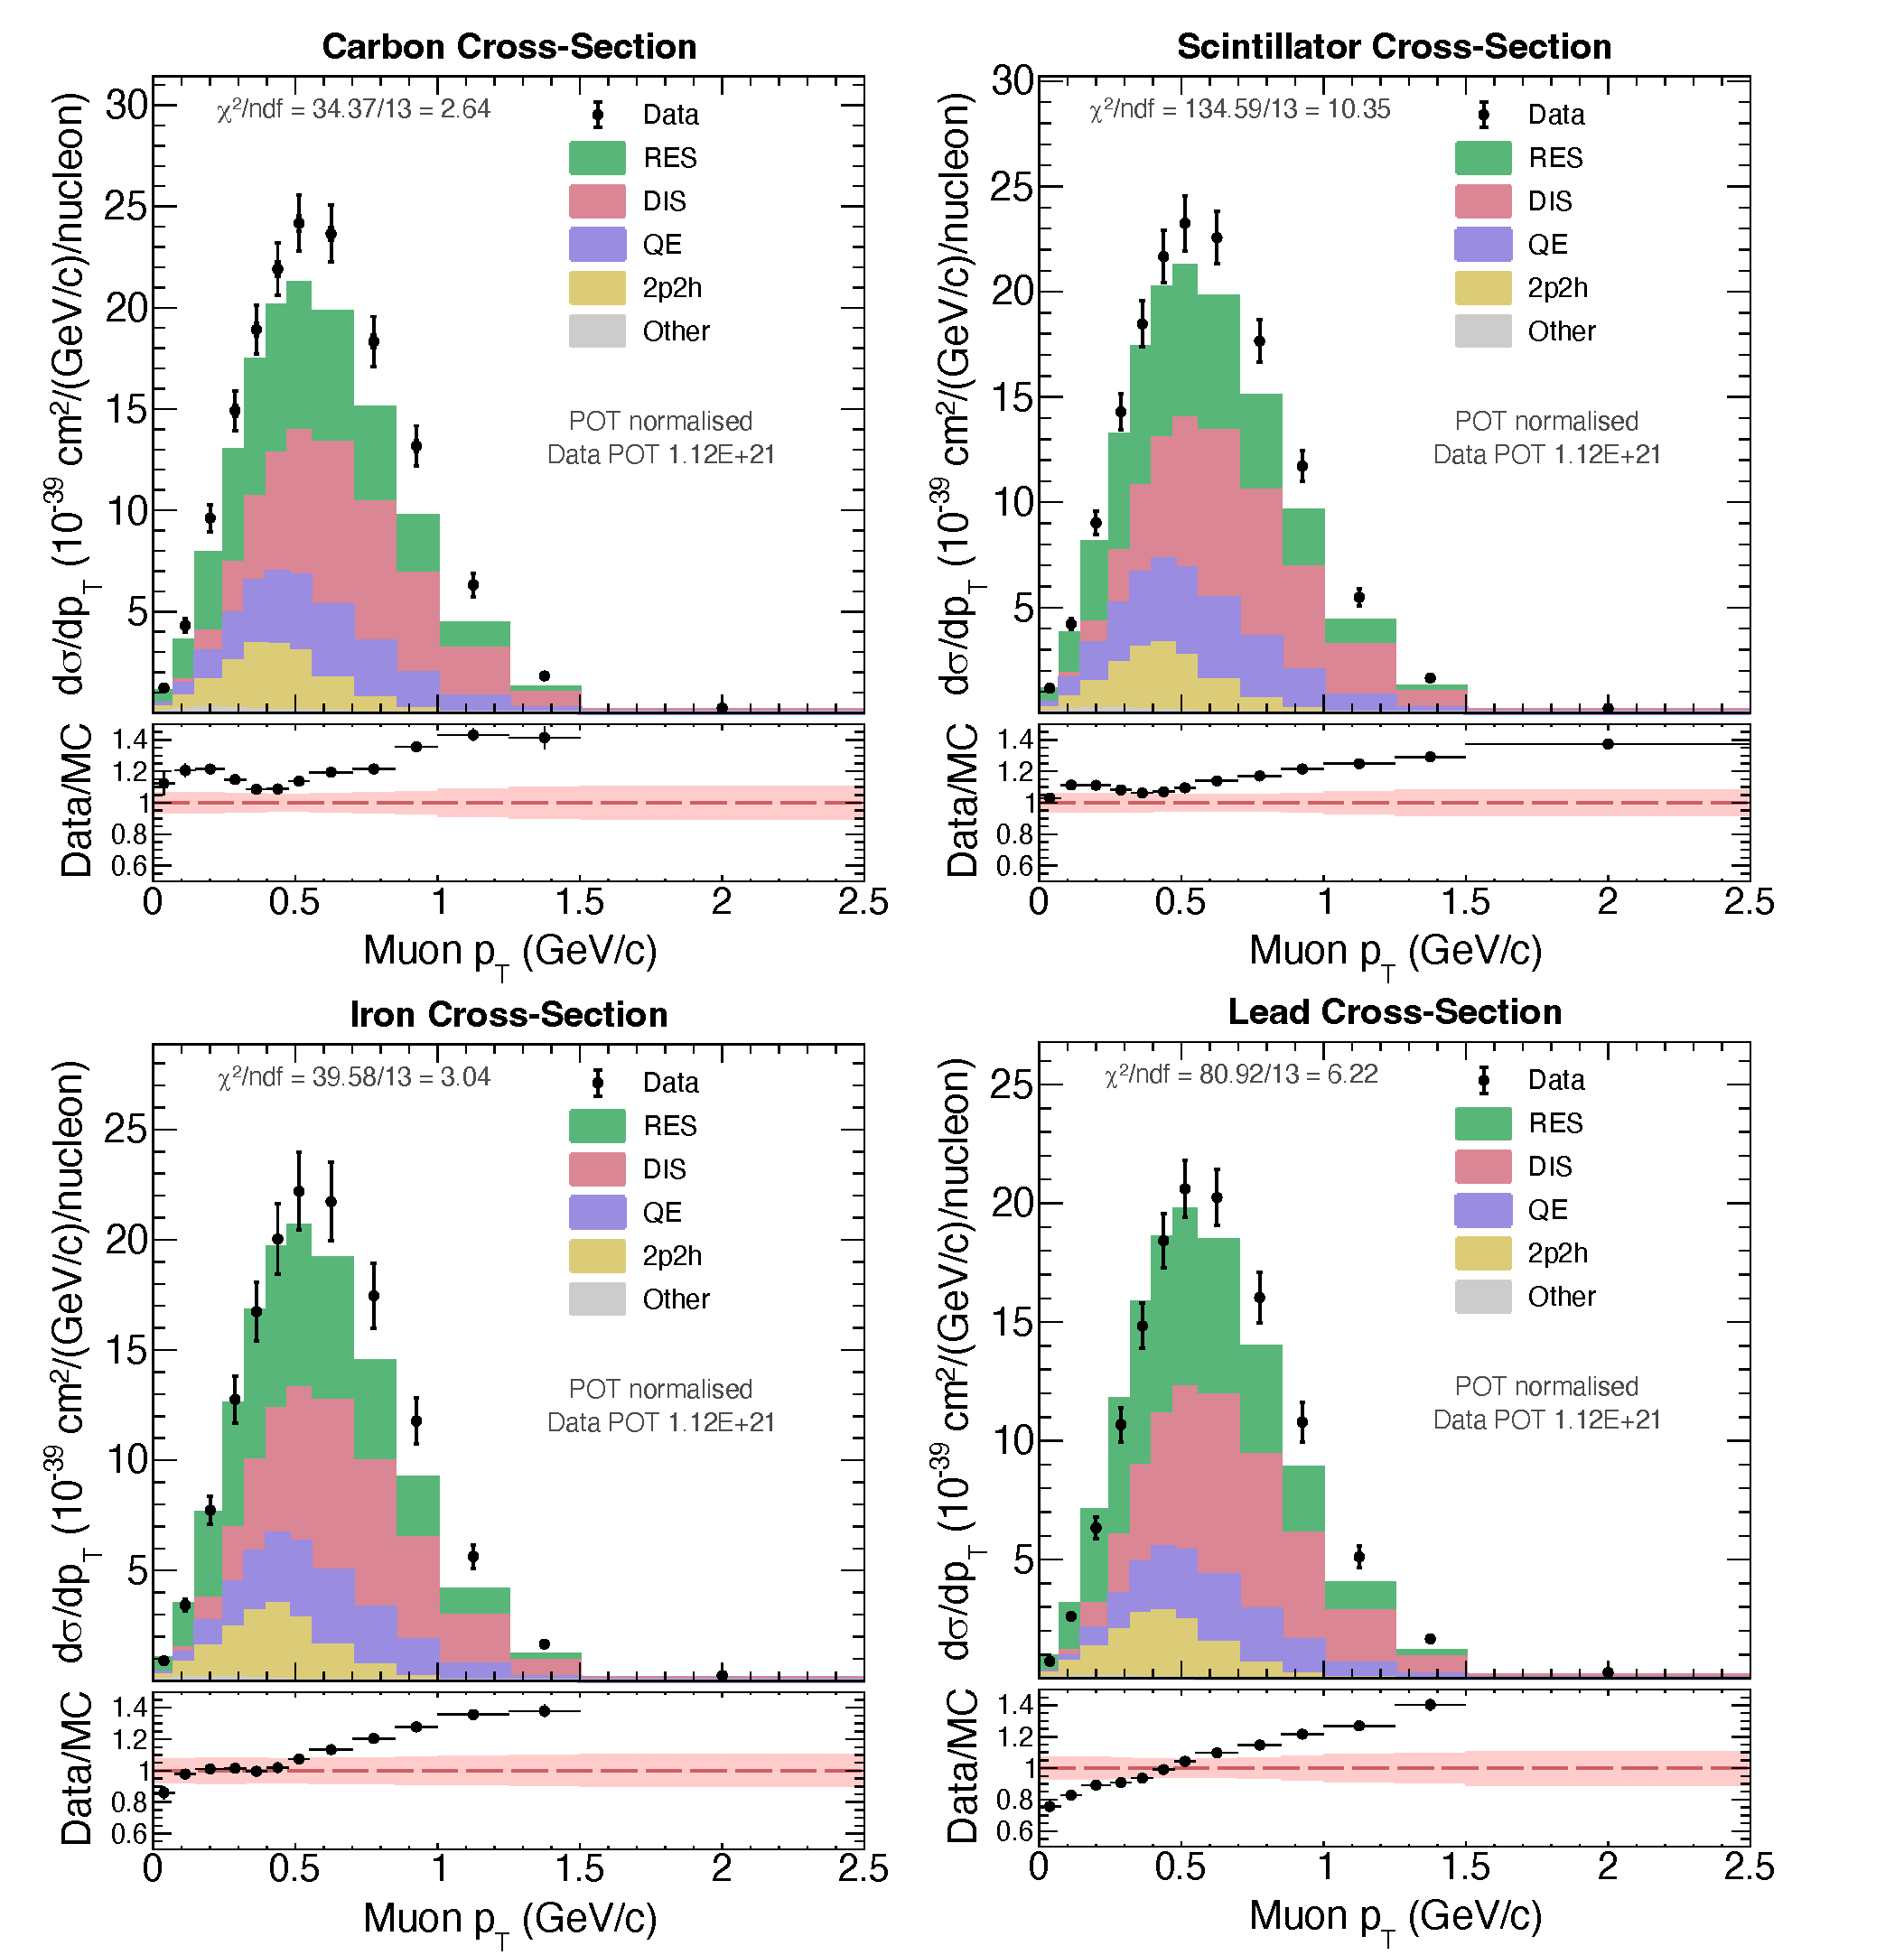
\includegraphics[width=1.\textwidth]{09results/figures/xsec_pT.pdf}}%
    \caption{Carbon, scintillator, iron, and lead (from left to right, top to bottom) cross-section as a function of $p_{\text{T}}$ with the simulation broken down into the various interaction channels stacked in the descending order of their contribution. In the top panel of each plot, the data points carry both statistical (inner error bar) and systematic (outer error bar, which is the sum of statistical and systematic errors) uncertainties. The bottom panel of each plot displays the data-to-simulation ratio, with the pink band around 1 representing systematic uncertainty on the data, while the black points reflect the statistical uncertainty on the data-to-simulation ratio.}
    \label{fig:xsec_pT}
\end{figure}


Importantly, the data-to-simulation ratios in Figure~\ref{fig:xsec_pT} reflect the trend observed throughout the analysis process. The region from the falling edge of the $p_{\text{T}}$ distribution to large $p_{\text{T}}$ is systematically underpredicted by the simulation for all nuclei. The data excess grows as $p_{\text{T}}$ increases. Interestingly, a similar excess was reported in MINERvA's measurement of antineutrino quasi-elastic-like scattering only~\cite{PhysRevD.108.032018}. This indicates that either quasi-elastic scattering or resonant pion production, or a combination thereof, is being mismodelled, i.e. underpredicted, by the underlying simulation. 


Furthermore, the low $p_{\text{T}}$ region presents an interesting insight into the nuclear dependence of the inclusive antineutrino scattering, which is mostly ascribed to the resonant pion production in the simulation. The simulation prediction ranges from underprediction of the data for relatively light nuclei, i.e. low-$A$ carbon and hydrocarbon, to significant overprediction of the data for high-$A$ lead. In other words, the discrepancy changes and grows as a function of the mass number $A$. Notably, this has been seen in MINERvA's medium-energy neutrino charged-current single $\pi^+$ production on various nuclear targets~\cite{Bercellie2023_PhysRevLett.131.011801}. The low $Q^2$ suppression was also featured in several other datasets including MINOS neutrino measurement on iron~\cite{PhysRevD.91.012005}, and MINERvA low-energy measurements of neutrino pion production on the scintillator~\cite{PhysRevD.92.092008, PhysRevD.94.052005, PhysRevD.96.072003, PhysRevD.100.072005} and one low-energy antineutrino pion induced production also on the scintillator~\cite{PhysRevD.94.052005}. This analysis' result is the first such observation in an antineutrino dataset in medium energy across various nuclei. 

% RATIOS
\begin{figure}[t!] 
    \centering
    {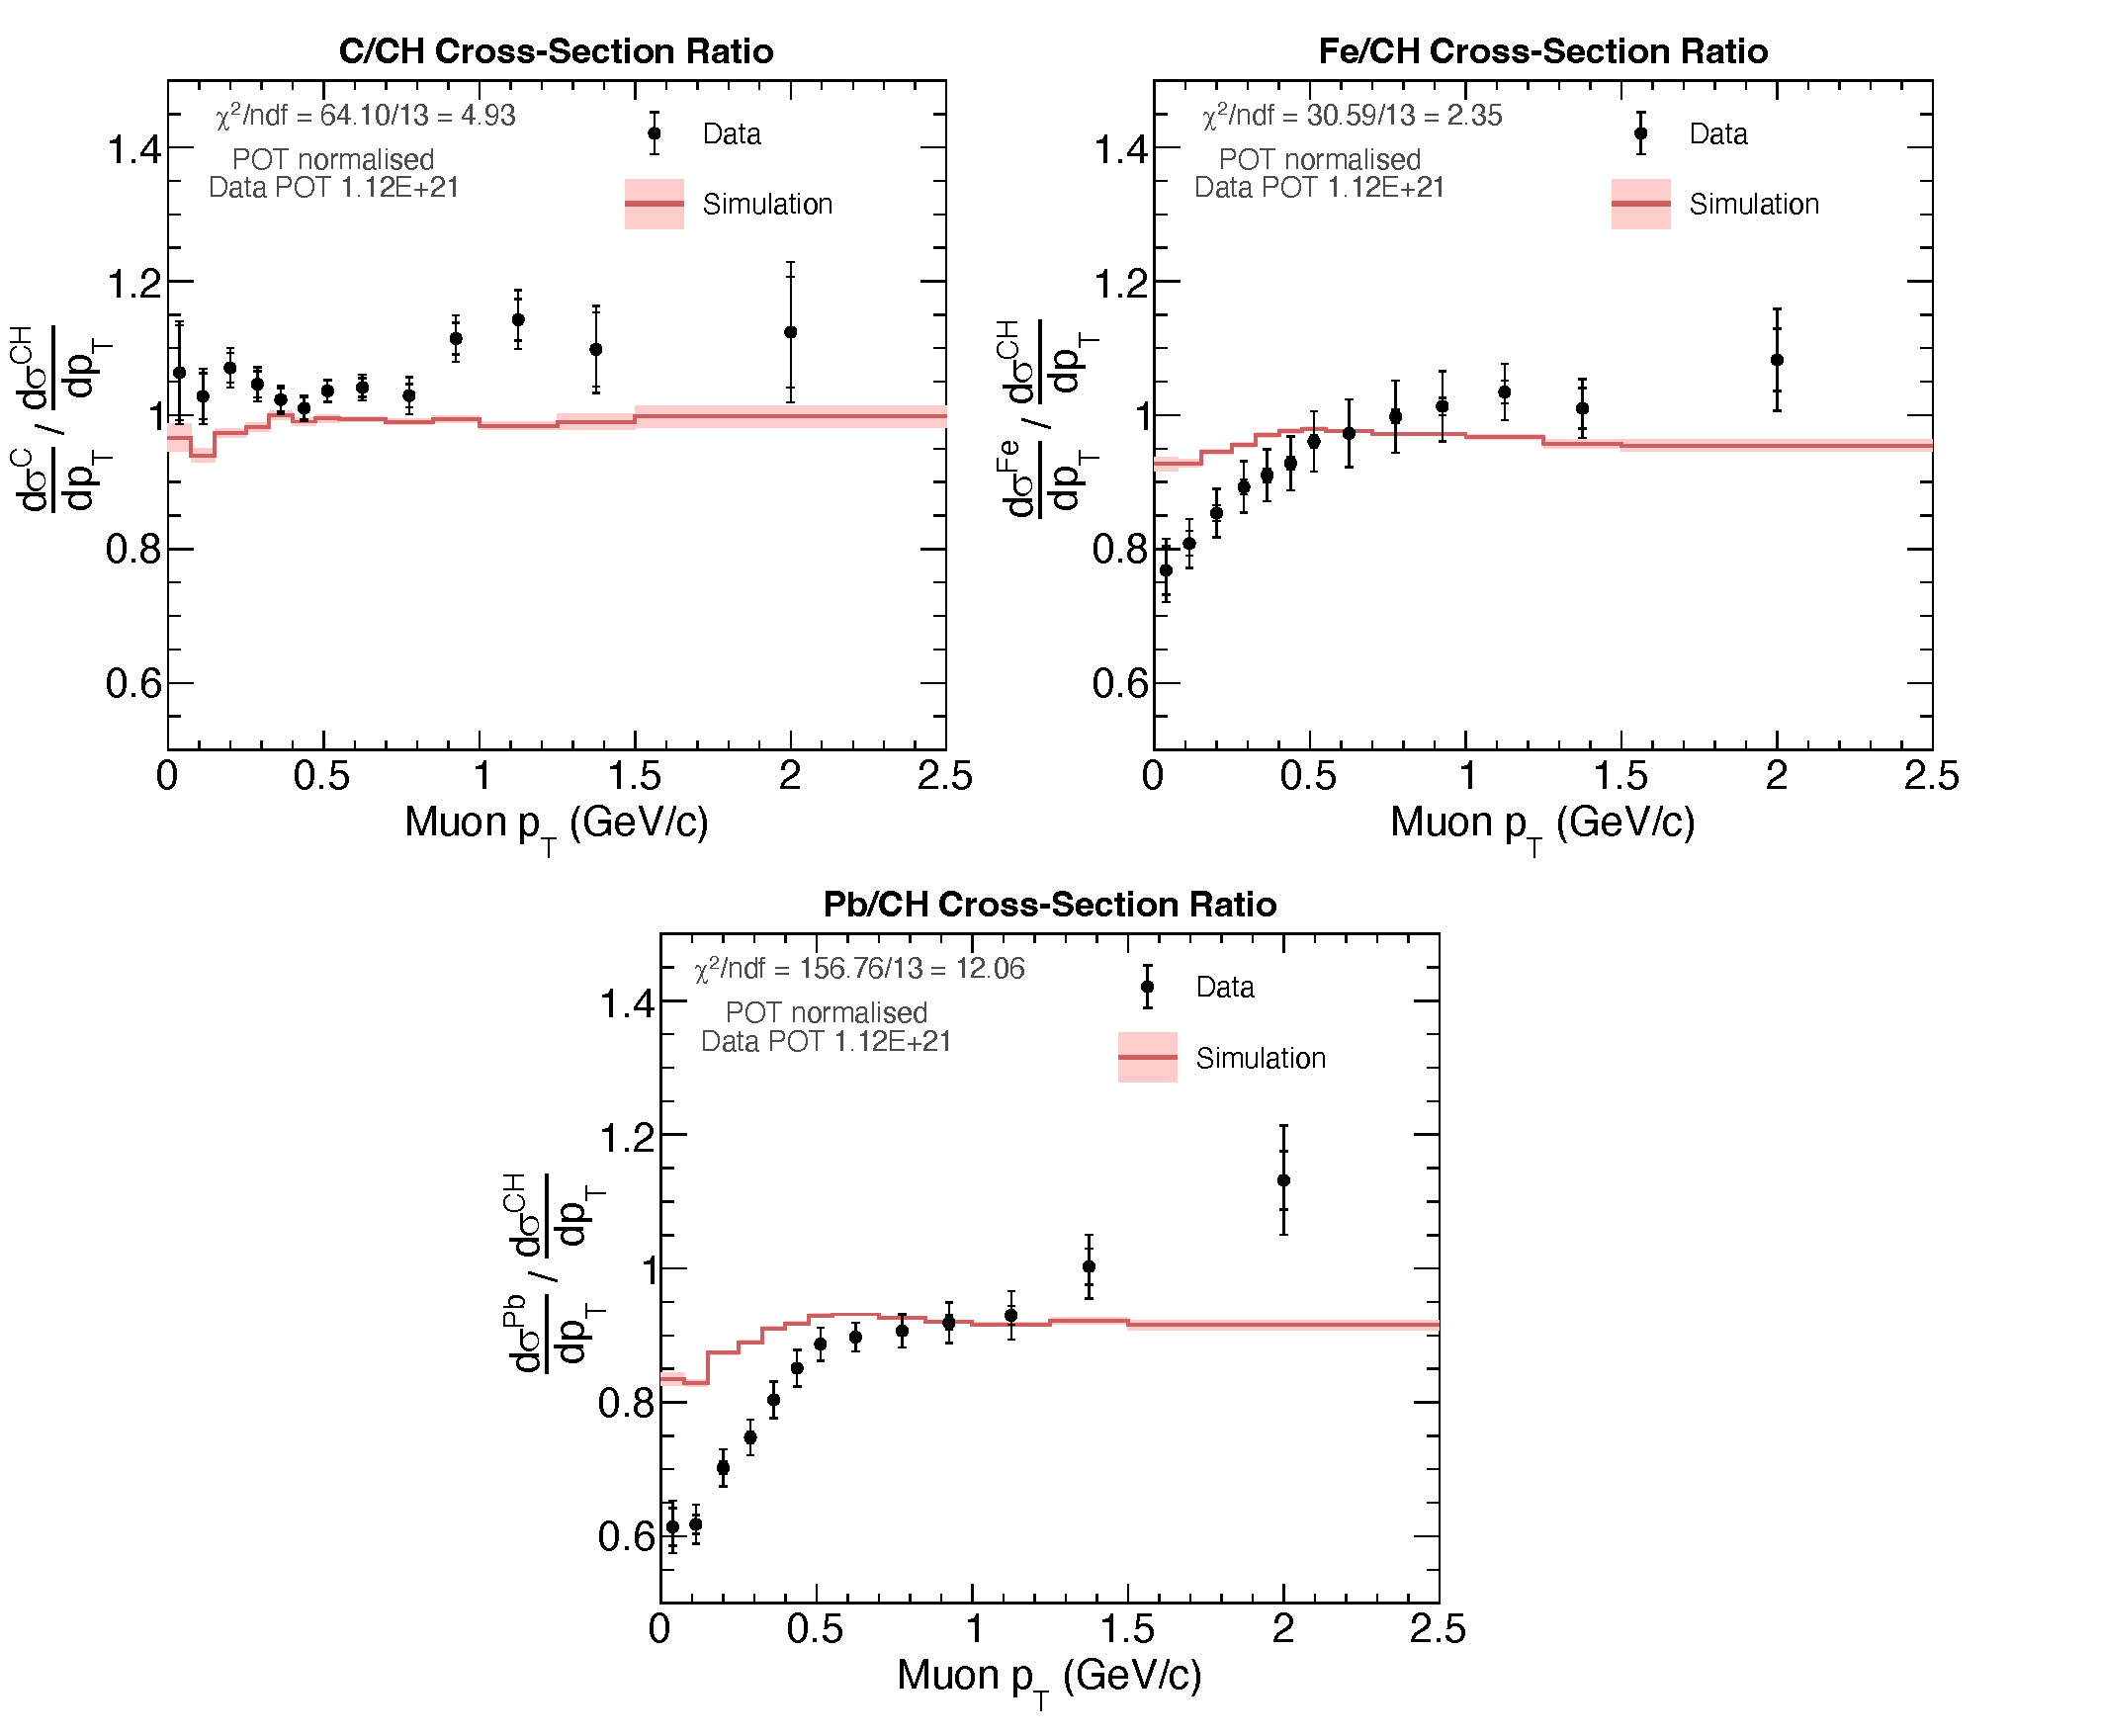
\includegraphics[width=1.\textwidth]{09results/figures/ratios_pT.pdf}}%
    \caption{Carbon-to-scintillator (top left), iron-to-scintillator (top right), and lead-to-scintillator (bottom) cross-section ratios in antimuon $p_{\text{T}}$. The data points carry both statistical (inner error bar) and systematic (outer error bar, which is the sum of statistical and systematic errors) uncertainties. The error band around the simulation predictions represents its statistical error. Note the significant $A$-dependence across the measured ratios, particularly in the low-$p_{\text{T}}$ region.}
    \label{fig:ratio_pT}
\end{figure}

As described in Chapter~\ref{ch:dataAsimulation}, this analysis tried to partially remedy the suppression by reweighting its single pion production, both resonant and non-resonant, with $\pi^-$ in final states, to match the low $Q^2$ (low $p_{\text{T}}$) suppression observed in the medium-energy single $\pi^+$ production on scintillator~\cite{Bercellie2023_PhysRevLett.131.011801}. While
the interpolation from neutrino to antineutrino mode was not necessarily expected to work, the suppression improved the simulation agreement with the data which is demonstrated in Appendix~\ref{ch:appendix_tuneComparisons}. The results show that this suppression seems to partially capture antineutrino interactions on iron, but it is not strong enough for lead. 

These observed trends are further amplified by looking at the carbon-, iron-, and lead-to-scintillator ratios in Figure~\ref{fig:ratio_pT}. While the carbon-to-scintillator ratio in antimuon $p_{\text{T}}$ is relatively flat as expected, the iron-to-scintillator and lead-to-scintillator ratios demonstrate dramatic $A$-scaling changes as a function of $p_{\text{T}}$, specifically at low and high $p_{\text{T}}$ as mentioned above. Overall these results suggest that both the total cross-section scaling versus $A$ and the low $Q^2$ suppression are larger than modelled and that the effect increases with increasing $p_{\text{T}}$ (square of the four-momentum transfer). Crucially, while the low $Q^2$ suppression is based on the pion production measurements, the inclusive antineutrino analysis spans other interaction channels that may contribute to the suppression observed in this region.

\begin{figure}[t!] 
    \centering
    {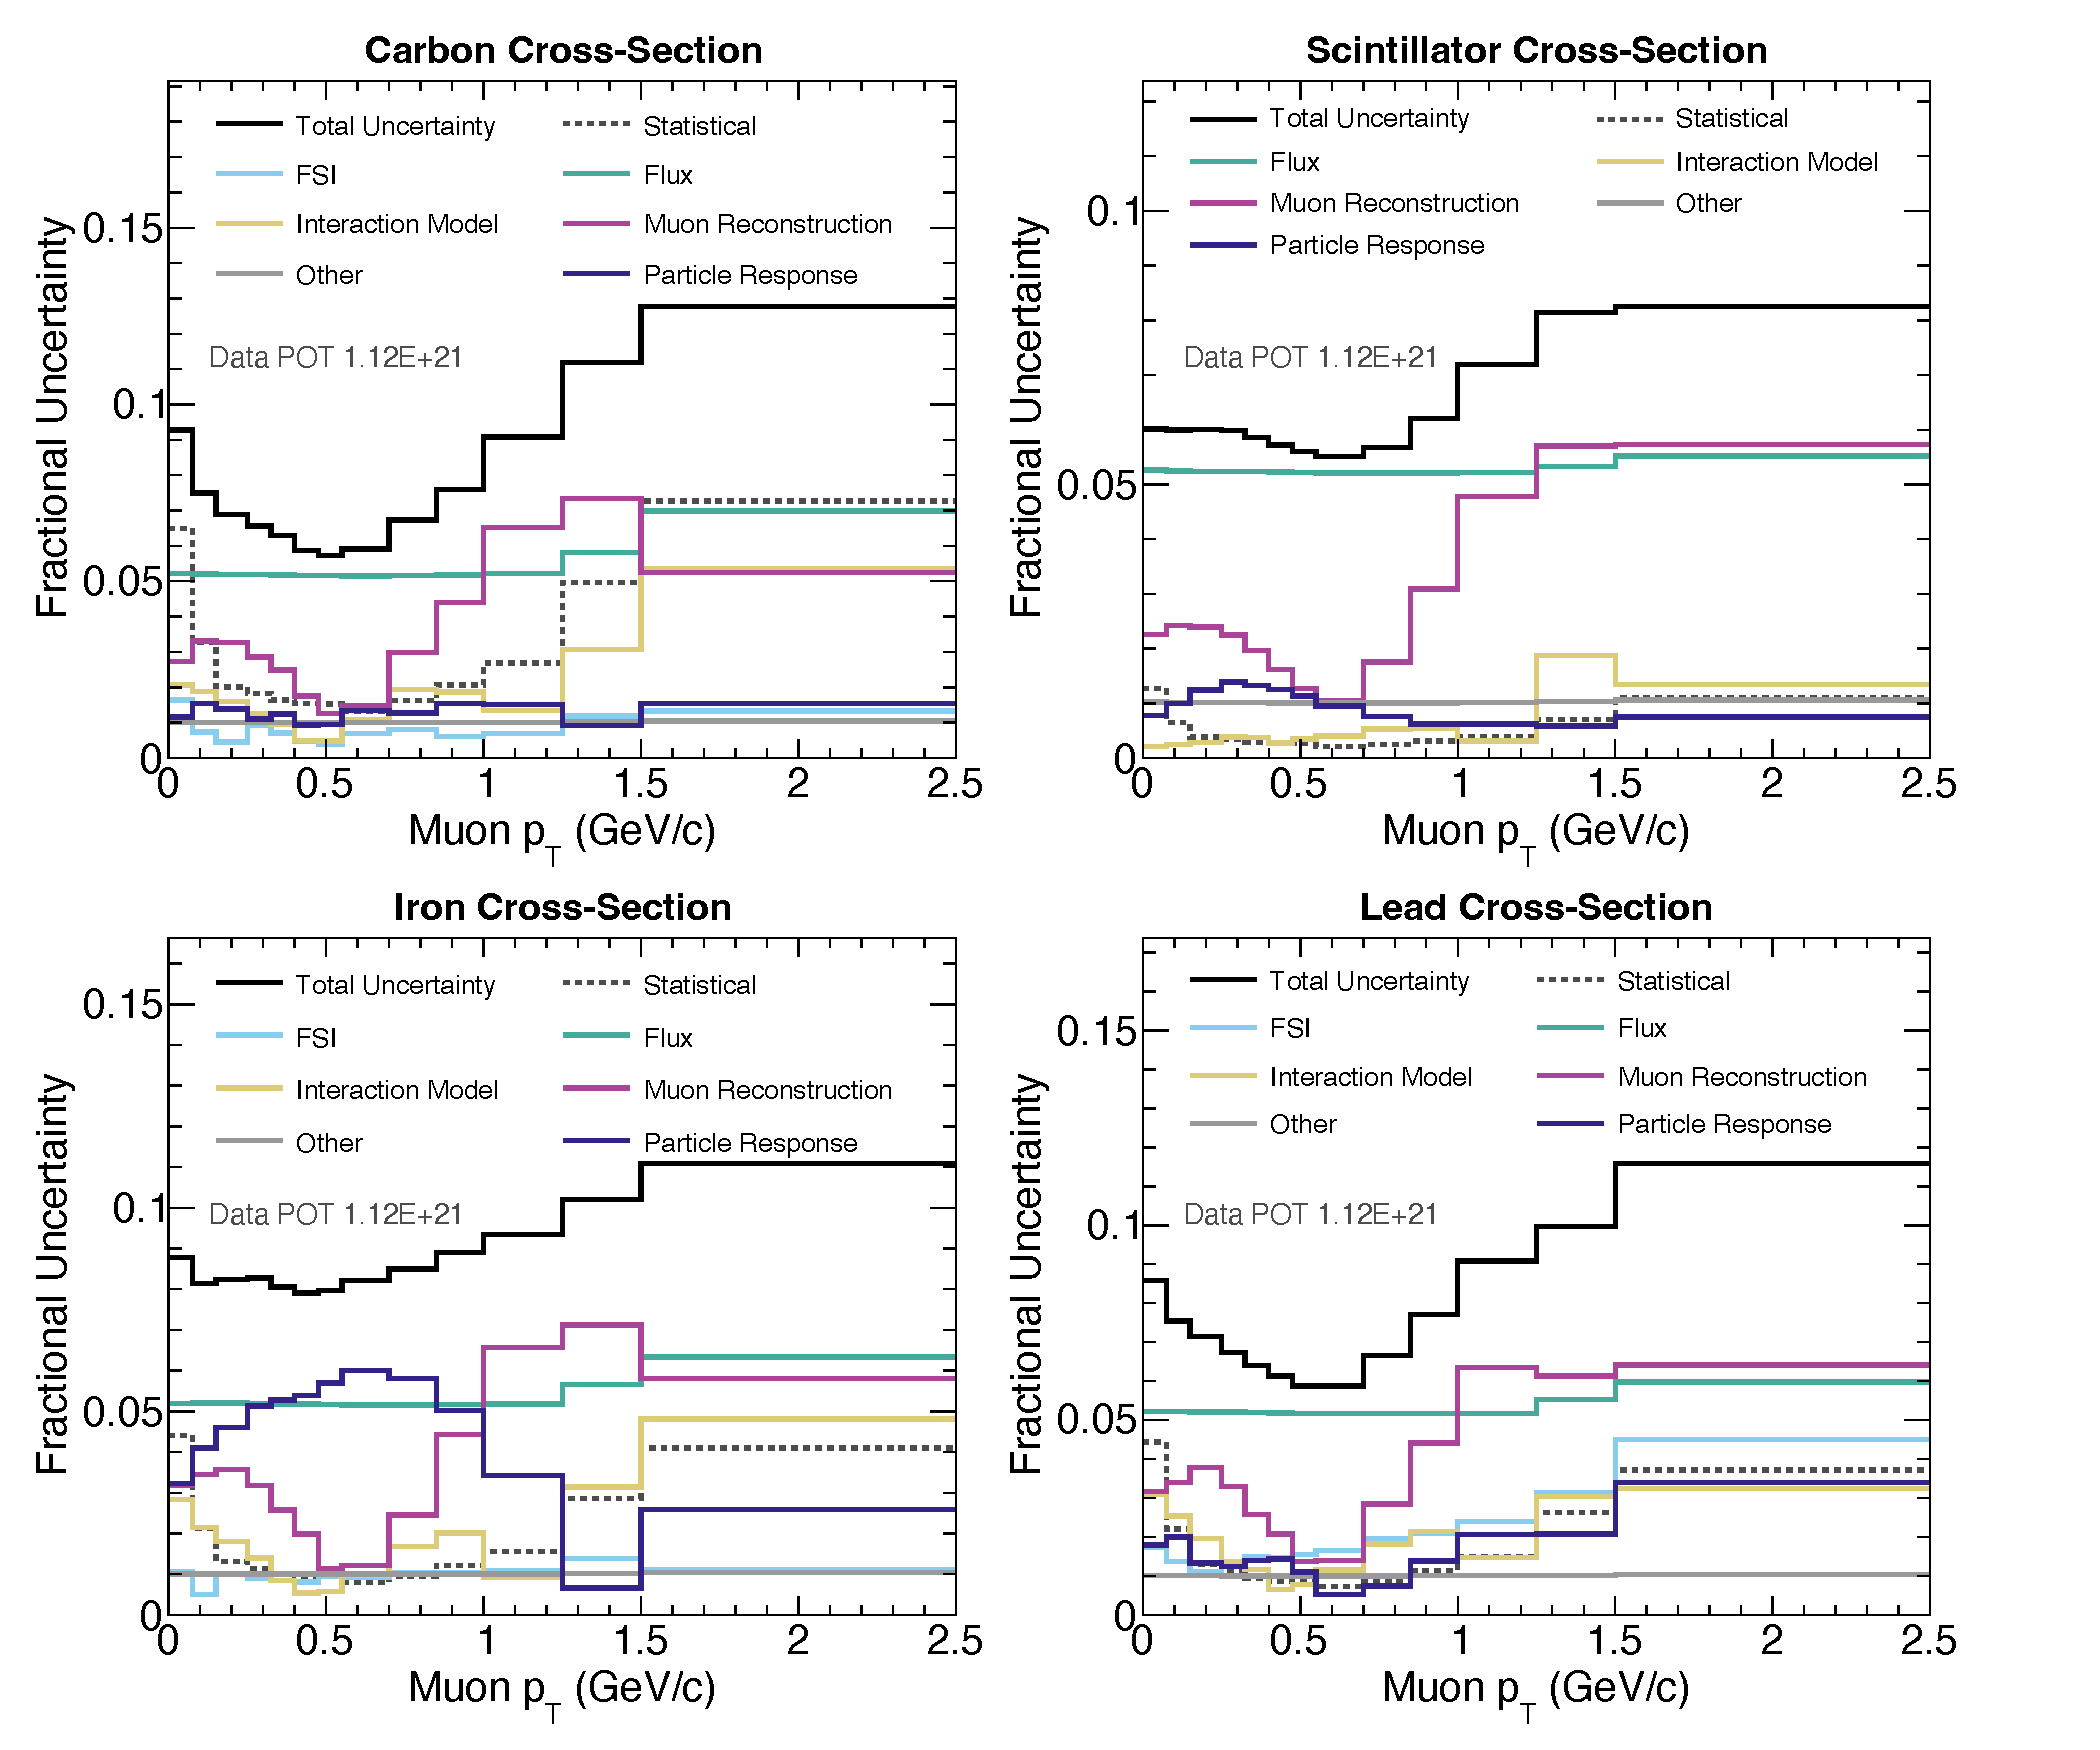
\includegraphics[width=1.\textwidth]{09results/figures/xsec_pT_fracErr.pdf}}%
    \caption{Breakdown of the fractional uncertainties on the data cross-section in $p_{\text{T}}$ for carbon, hydrocarbon, iron, and lead (from left to right, top to bottom). Note that the cross-sections are dominated by the uncertainties on flux and antimuon reconstruction.}
    \label{fig:xsec_pT_fracErr}
\end{figure}

An interesting observation is the flat carbon-to-scintillator ratio in Figure~\ref{fig:ratio_pT}, which does not completely agree with the simulation prediction at unity, contrary to expectations. However, it is important to note that the systematic uncertainties on the data are missing the uncertainty accounting for the discrepancy in the plastic sidebands after the normalisation tune discussed in Section~\ref{sec:bkgSubtraction} and Chapter~\ref{ch:systematics}. Given that the shape of the ratio somewhat mirrors the shape of the data-to-simulation ratio in the sideband, this is expected to account for the discrepancy between the data and the simulation prediction in the final carbon-to-scintillator cross-section ratio. Alternatively, this discrepancy is also expected to be mitigated if the plastic sideband procedure is improved, for example, by fitting in the three distinct regions of $p_{\text{T}}$ (low, peak, and high $p_{\text{T}}$) to remove the shape differences in the sideband rather than using a simple normalisation fit. 

\begin{figure}[t!] 
    \centering
    {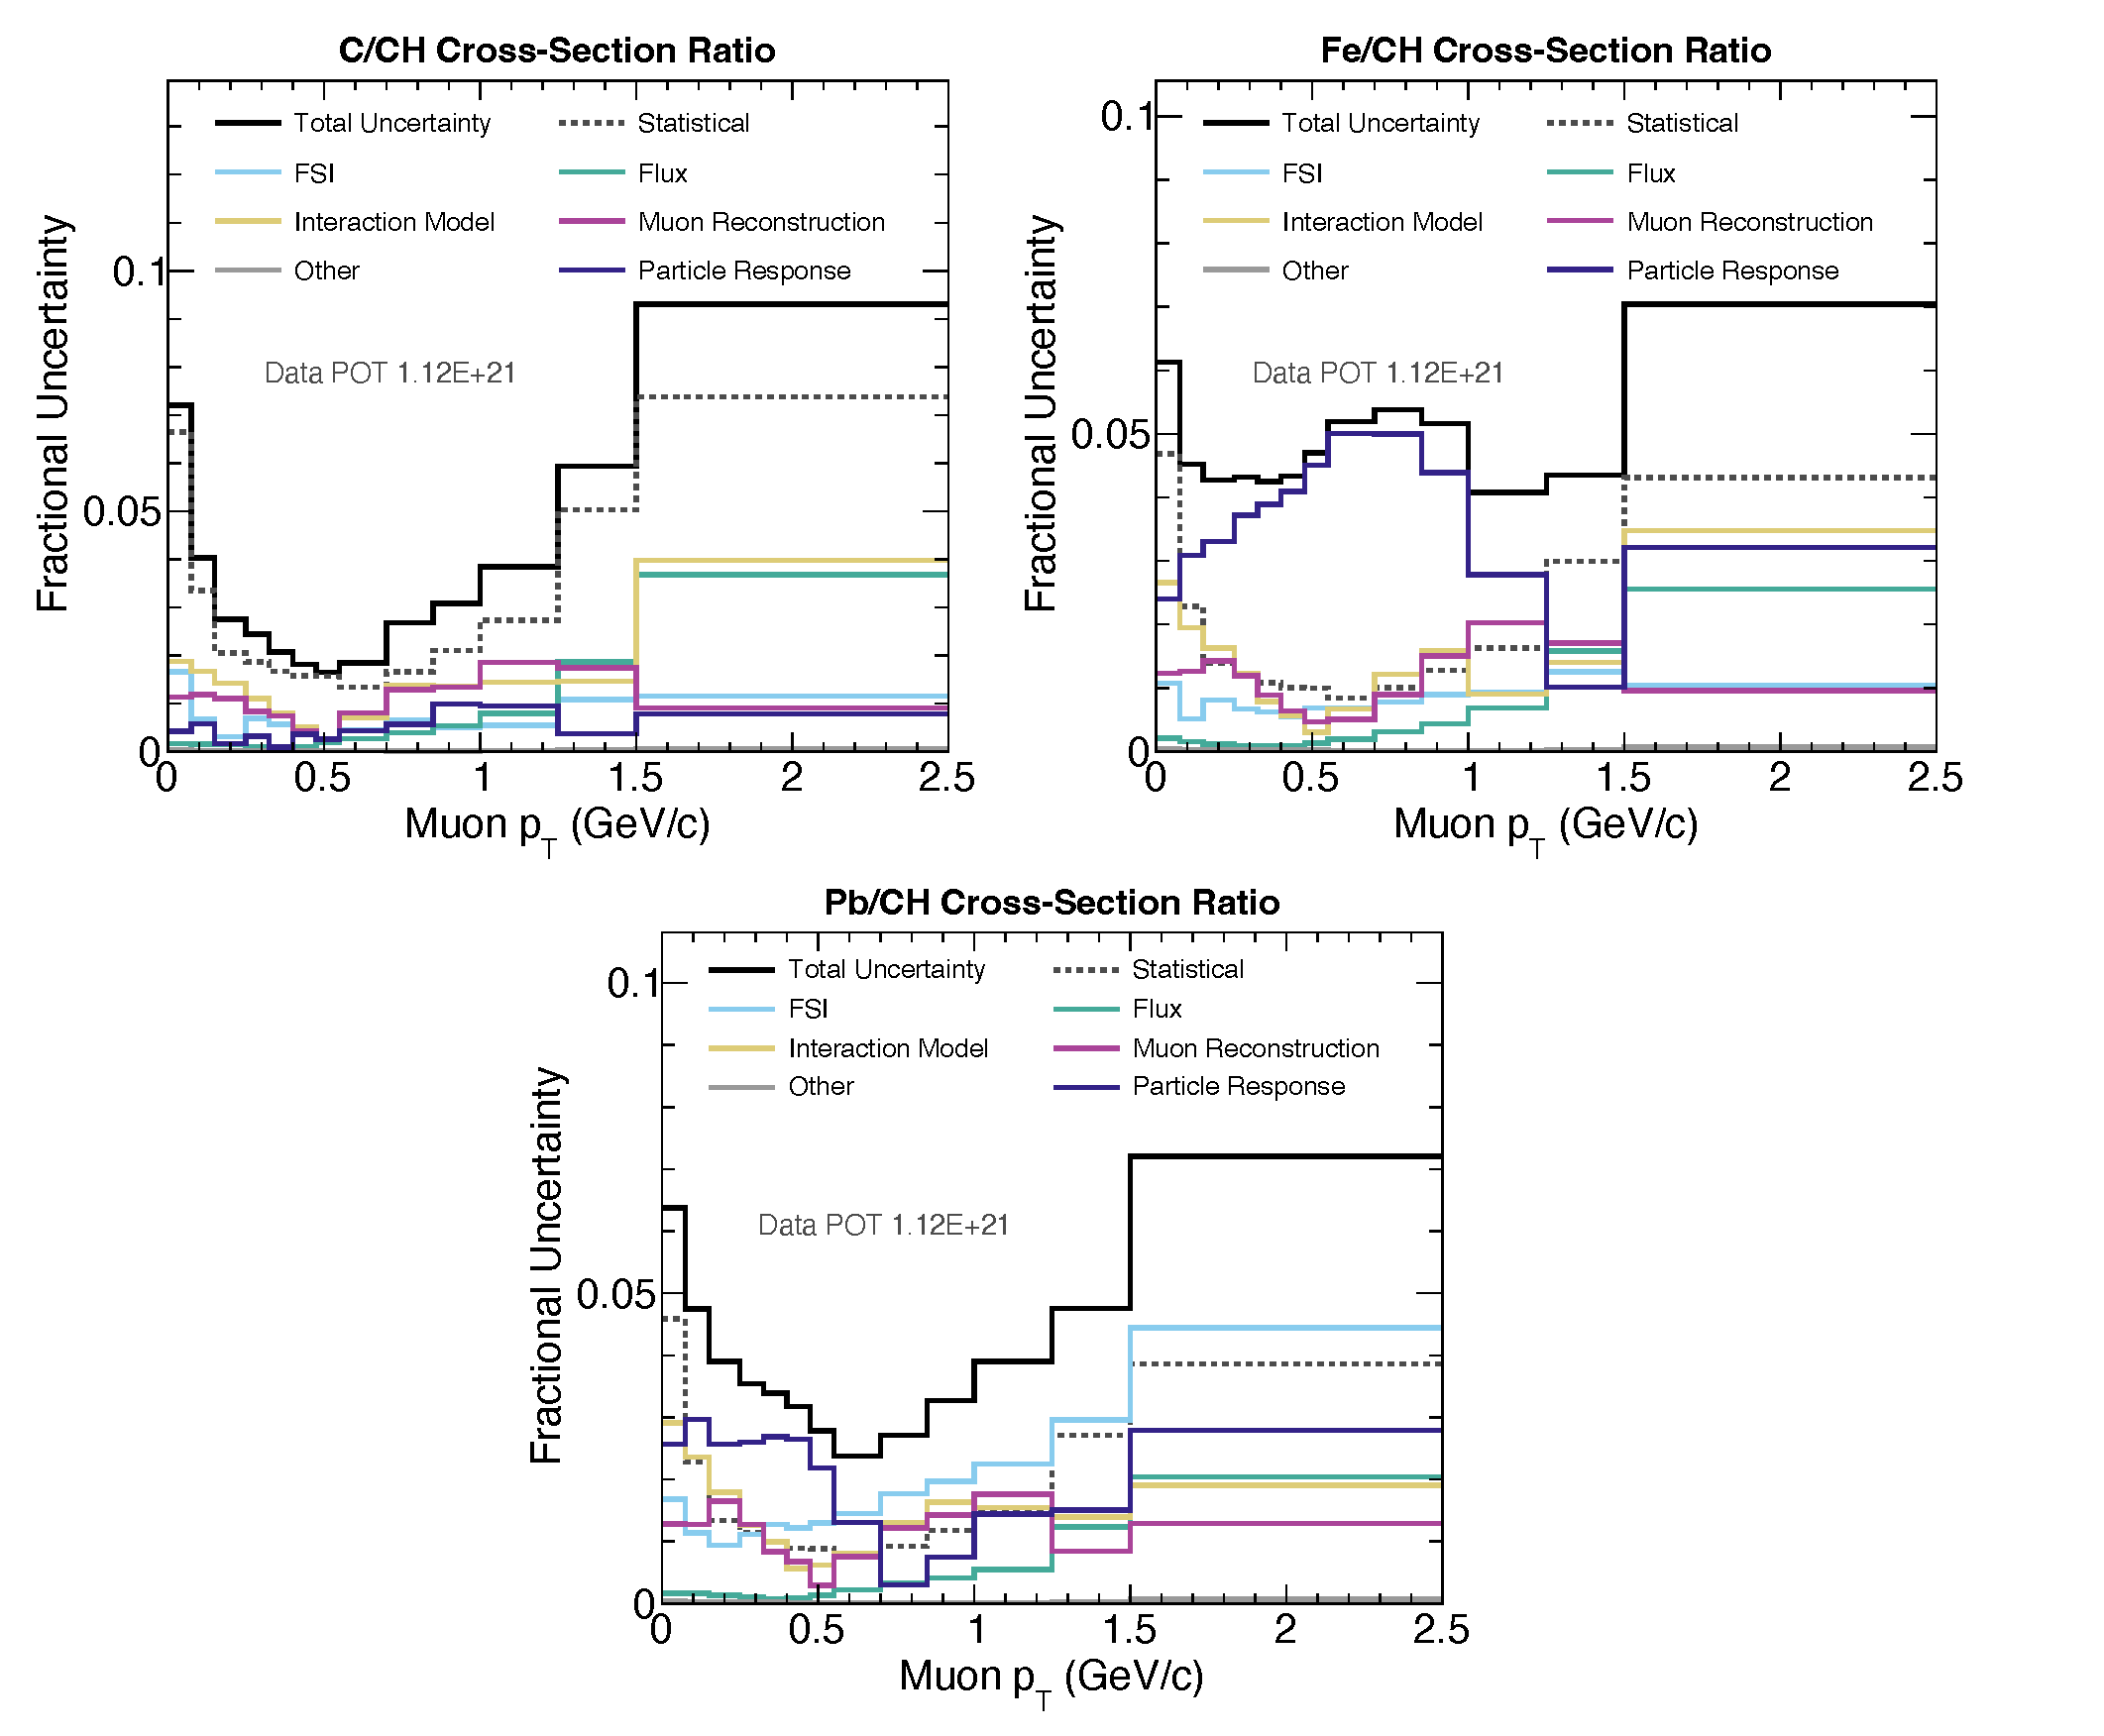
\includegraphics[width=1.\textwidth]{09results/figures/ratios_pT_fracErr.pdf}}%
    \caption{Breakdown of the fractional uncertainties on the data cross-section ratios to scintillator for carbon (top left), iron (top right), and lead (bottom) in antimuon $p_{\text{T}}$. Note that the flux and detector-related uncertainties are mostly cancelled out. A significant feature is the increase of the `FSI' error band going from light carbon to heavy lead. }
    \label{fig:ratio_pT_fracErr}
\end{figure}

Finally, the breakdowns of fractional uncertainties for both the cross-sections and cross-section ratios in $p_{\text{T}}$ are demonstrated in Figures~\ref{fig:xsec_pT_fracErr} and~\ref{fig:ratio_pT_fracErr}, respectively. The individual cross-sections are primarily influenced by systematic uncertainty rather than statistical uncertainty, specifically stemming from the flux and the antimuon reconstruction uncertainties. These two sources of uncertainty tend to cancel out to a large extent in the cross-section ratios, as evident in Figure~\ref{fig:ratio_pT_fracErr}. Consequently, the cross-section ratios become predominantly limited by statistical uncertainties.

When comparing C/CH, Fe/CH, and Pb/CH, a noticeable increase in the uncertainty on the final-state interaction~(`FSI') is observed as FSI becomes more significant and complex for heavier nuclei. It is important to note that the `Particle Response' uncertainty band is mainly driven by uncertainties in GEANT4 neutron interaction modelling, impacting the analysis due to correlations between outgoing particle kinematics (as $p_{\text{T}}$ serves as a proxy for the momentum transfer). A similar impact of the GEANT4 neutron modelling uncertainty in iron has been observed in other MINERvA analyses, such as in Ref.~\cite{Bercellie2023_PhysRevLett.131.011801}, and is currently under investigation, potentially arising from large weights in the neutron reweight described in Section~\ref{sec:particleProp}. %Note that the full covariance matrices for the measured antimuon $p_{\text{T}}$ cross-sections are included in Appendix~\ref{ch:appendix_covarianceMatrices}.
\clearpage
\section{Bjorken~$x$ results}


Figures~\ref{fig:xsec_x} and \ref{fig:ratio_x} show the results of the differential cross-sections and cross-section ratios for various nuclei as functions of the dimensionless scaling variable Bjorken $x$. As discussed in Chapter~\ref{ch:measurement}, Bjorken $x$ is used to describe nuclear modifications to a bound nucleon cross-section compared to a free nucleon. While this effect is primarily associated with deep inelastic scattering (DIS), the substantial DIS contribution in this analysis sample makes the investigation interesting. By definition, the DIS contribution is expected to be large at low $x$ (corresponding to large recoil energy), while the quasi-elastic contribution should dominate the high $x$ region. This is illustrated in the interaction breakdown of the simulation prediction cross-section in Figure~\ref{fig:xsec_x}.

\begin{figure}[t!] 
    \vspace{20pt}
    \centering
    {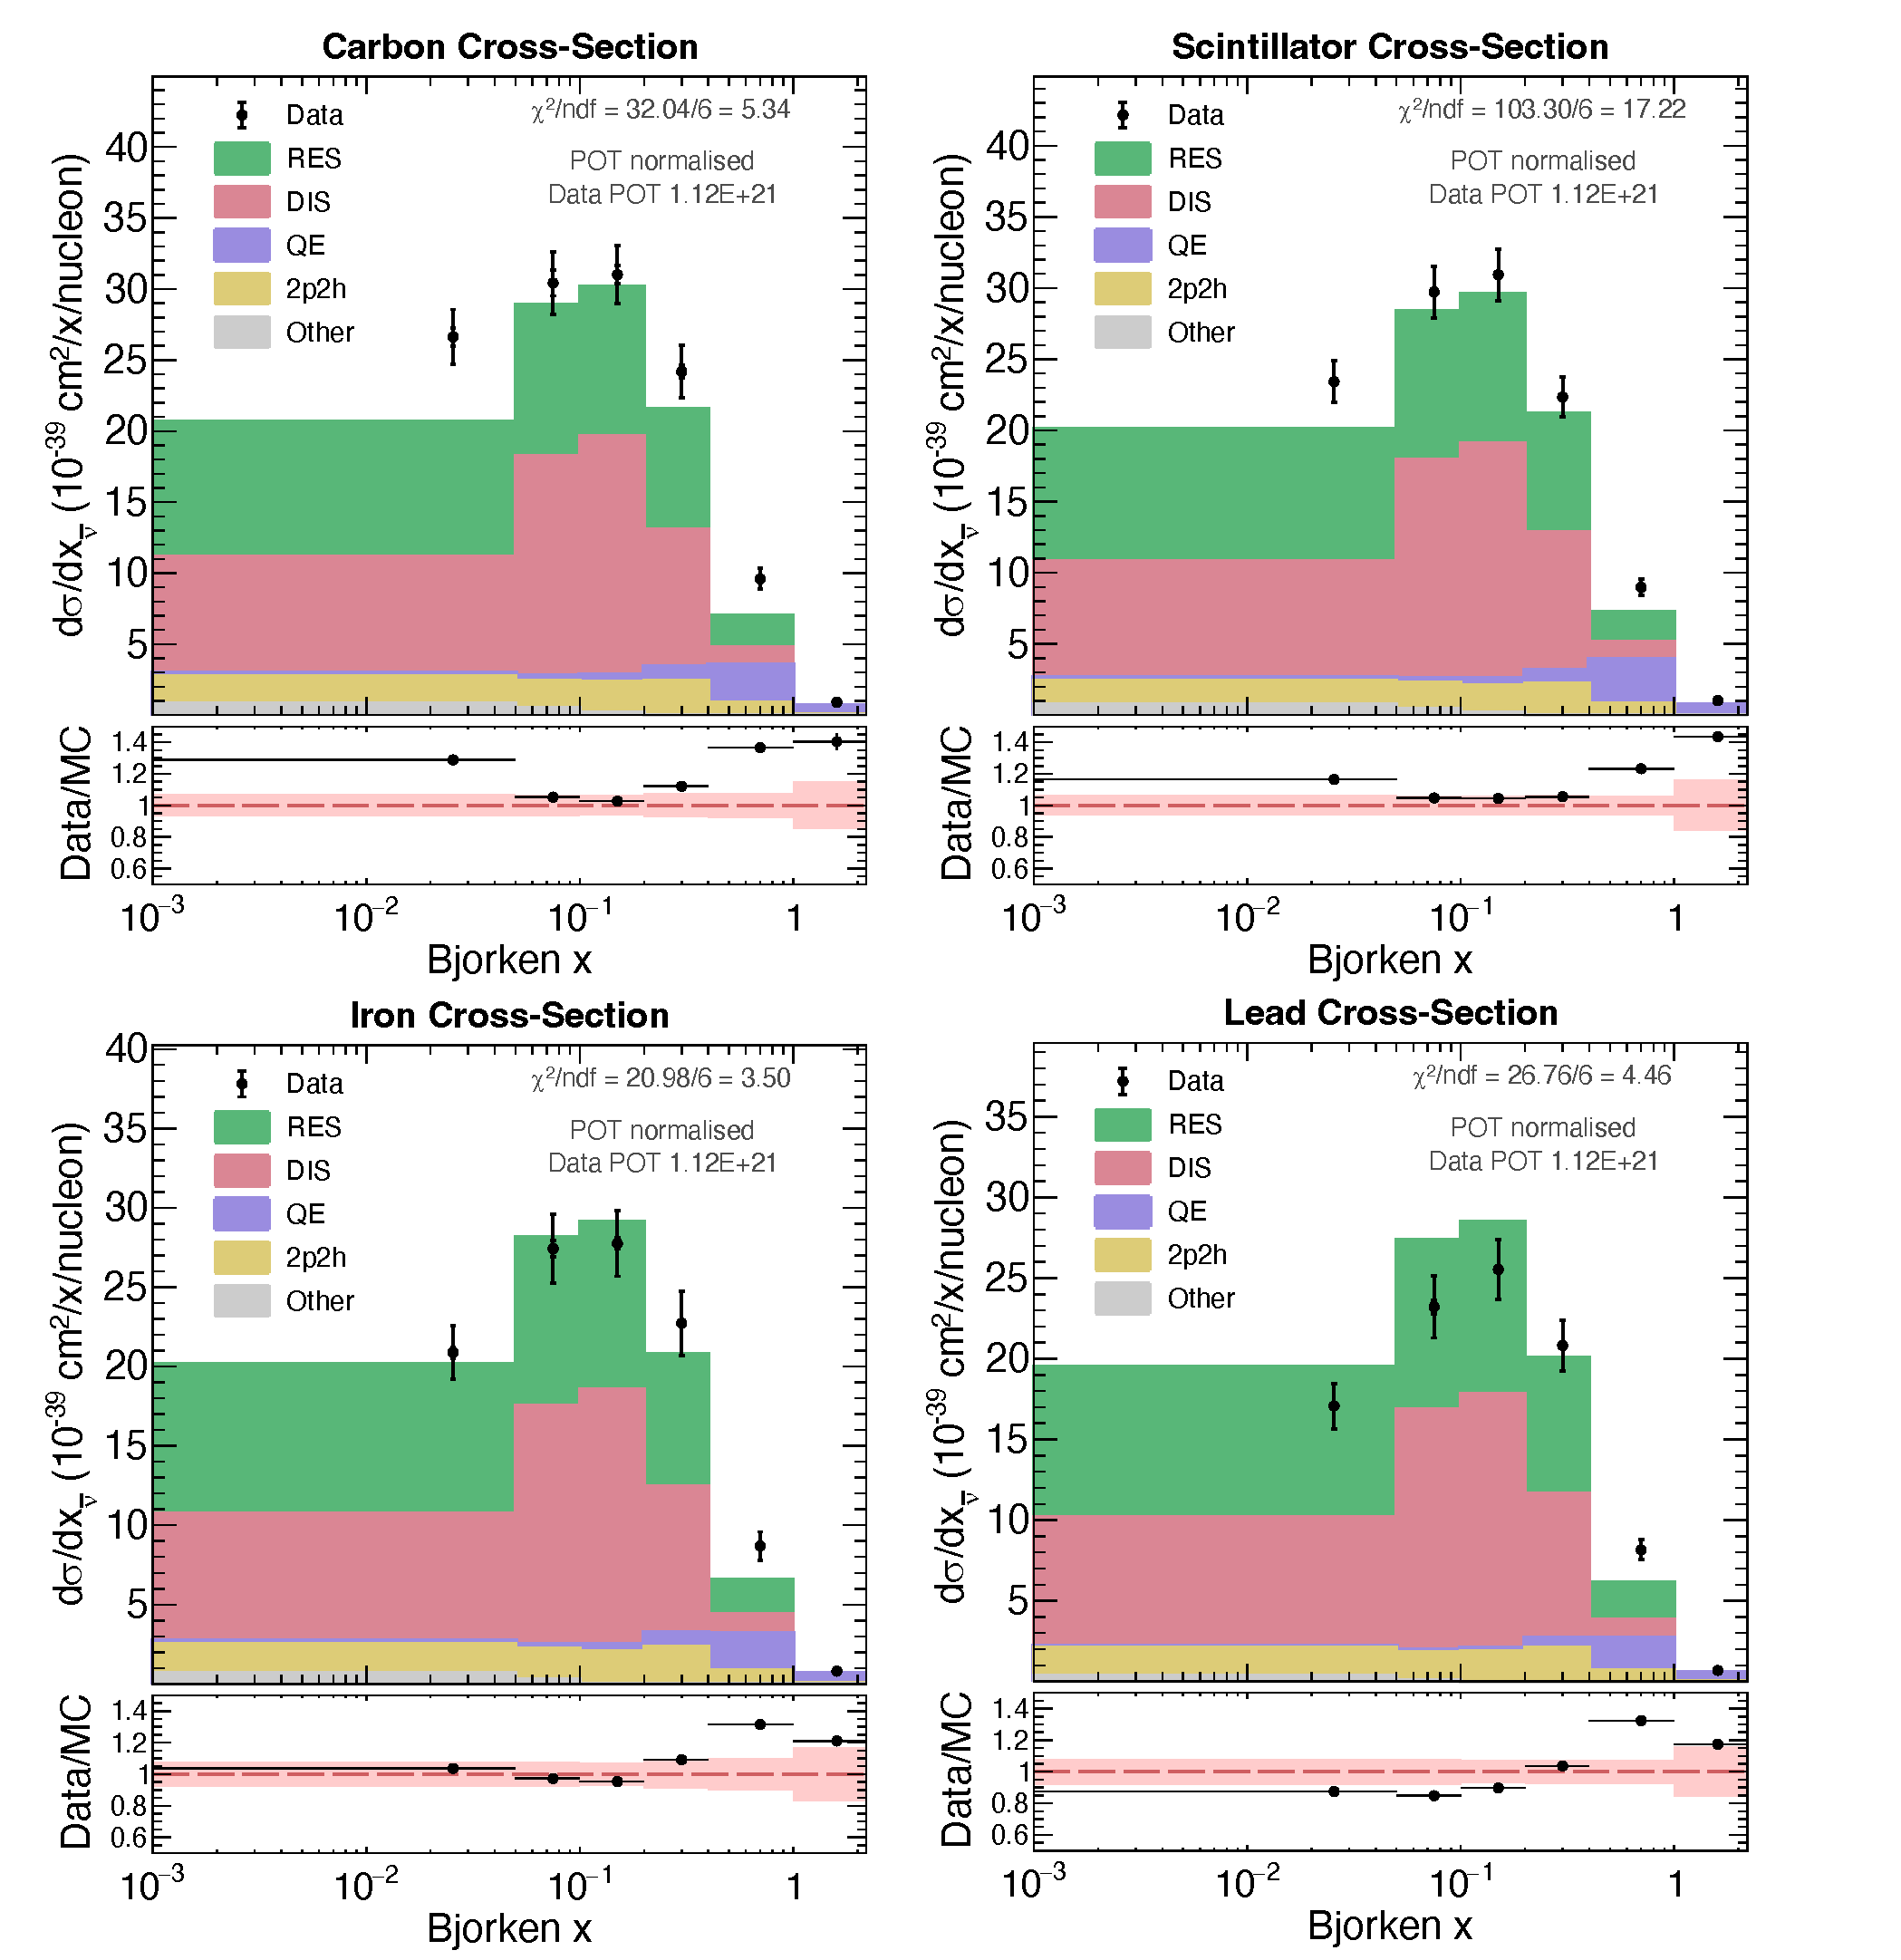
\includegraphics[width=1.\textwidth]{09results/figures/xsec_x.pdf}}%
    \caption{Carbon, scintillator, iron, and lead (from left to right, top to bottom) cross-section as a function of Bjorken $x$ with the simulation broken down into the various interaction channels stacked in the descending order of their contribution. In the top panel of each plot, the data points carry both statistical (inner error bar) and systematic (outer error bar, which is the sum of statistical and systematic errors) uncertainties. The bottom panel of each plot displays the data-to-simulation ratio, with the pink band around 1 representing systematic uncertainty on the data, while the black points reflect the statistical uncertainty on the data-to-simulation ratio.}
    \label{fig:xsec_x}
\end{figure}




\begin{figure}[t!] 
    \centering
    {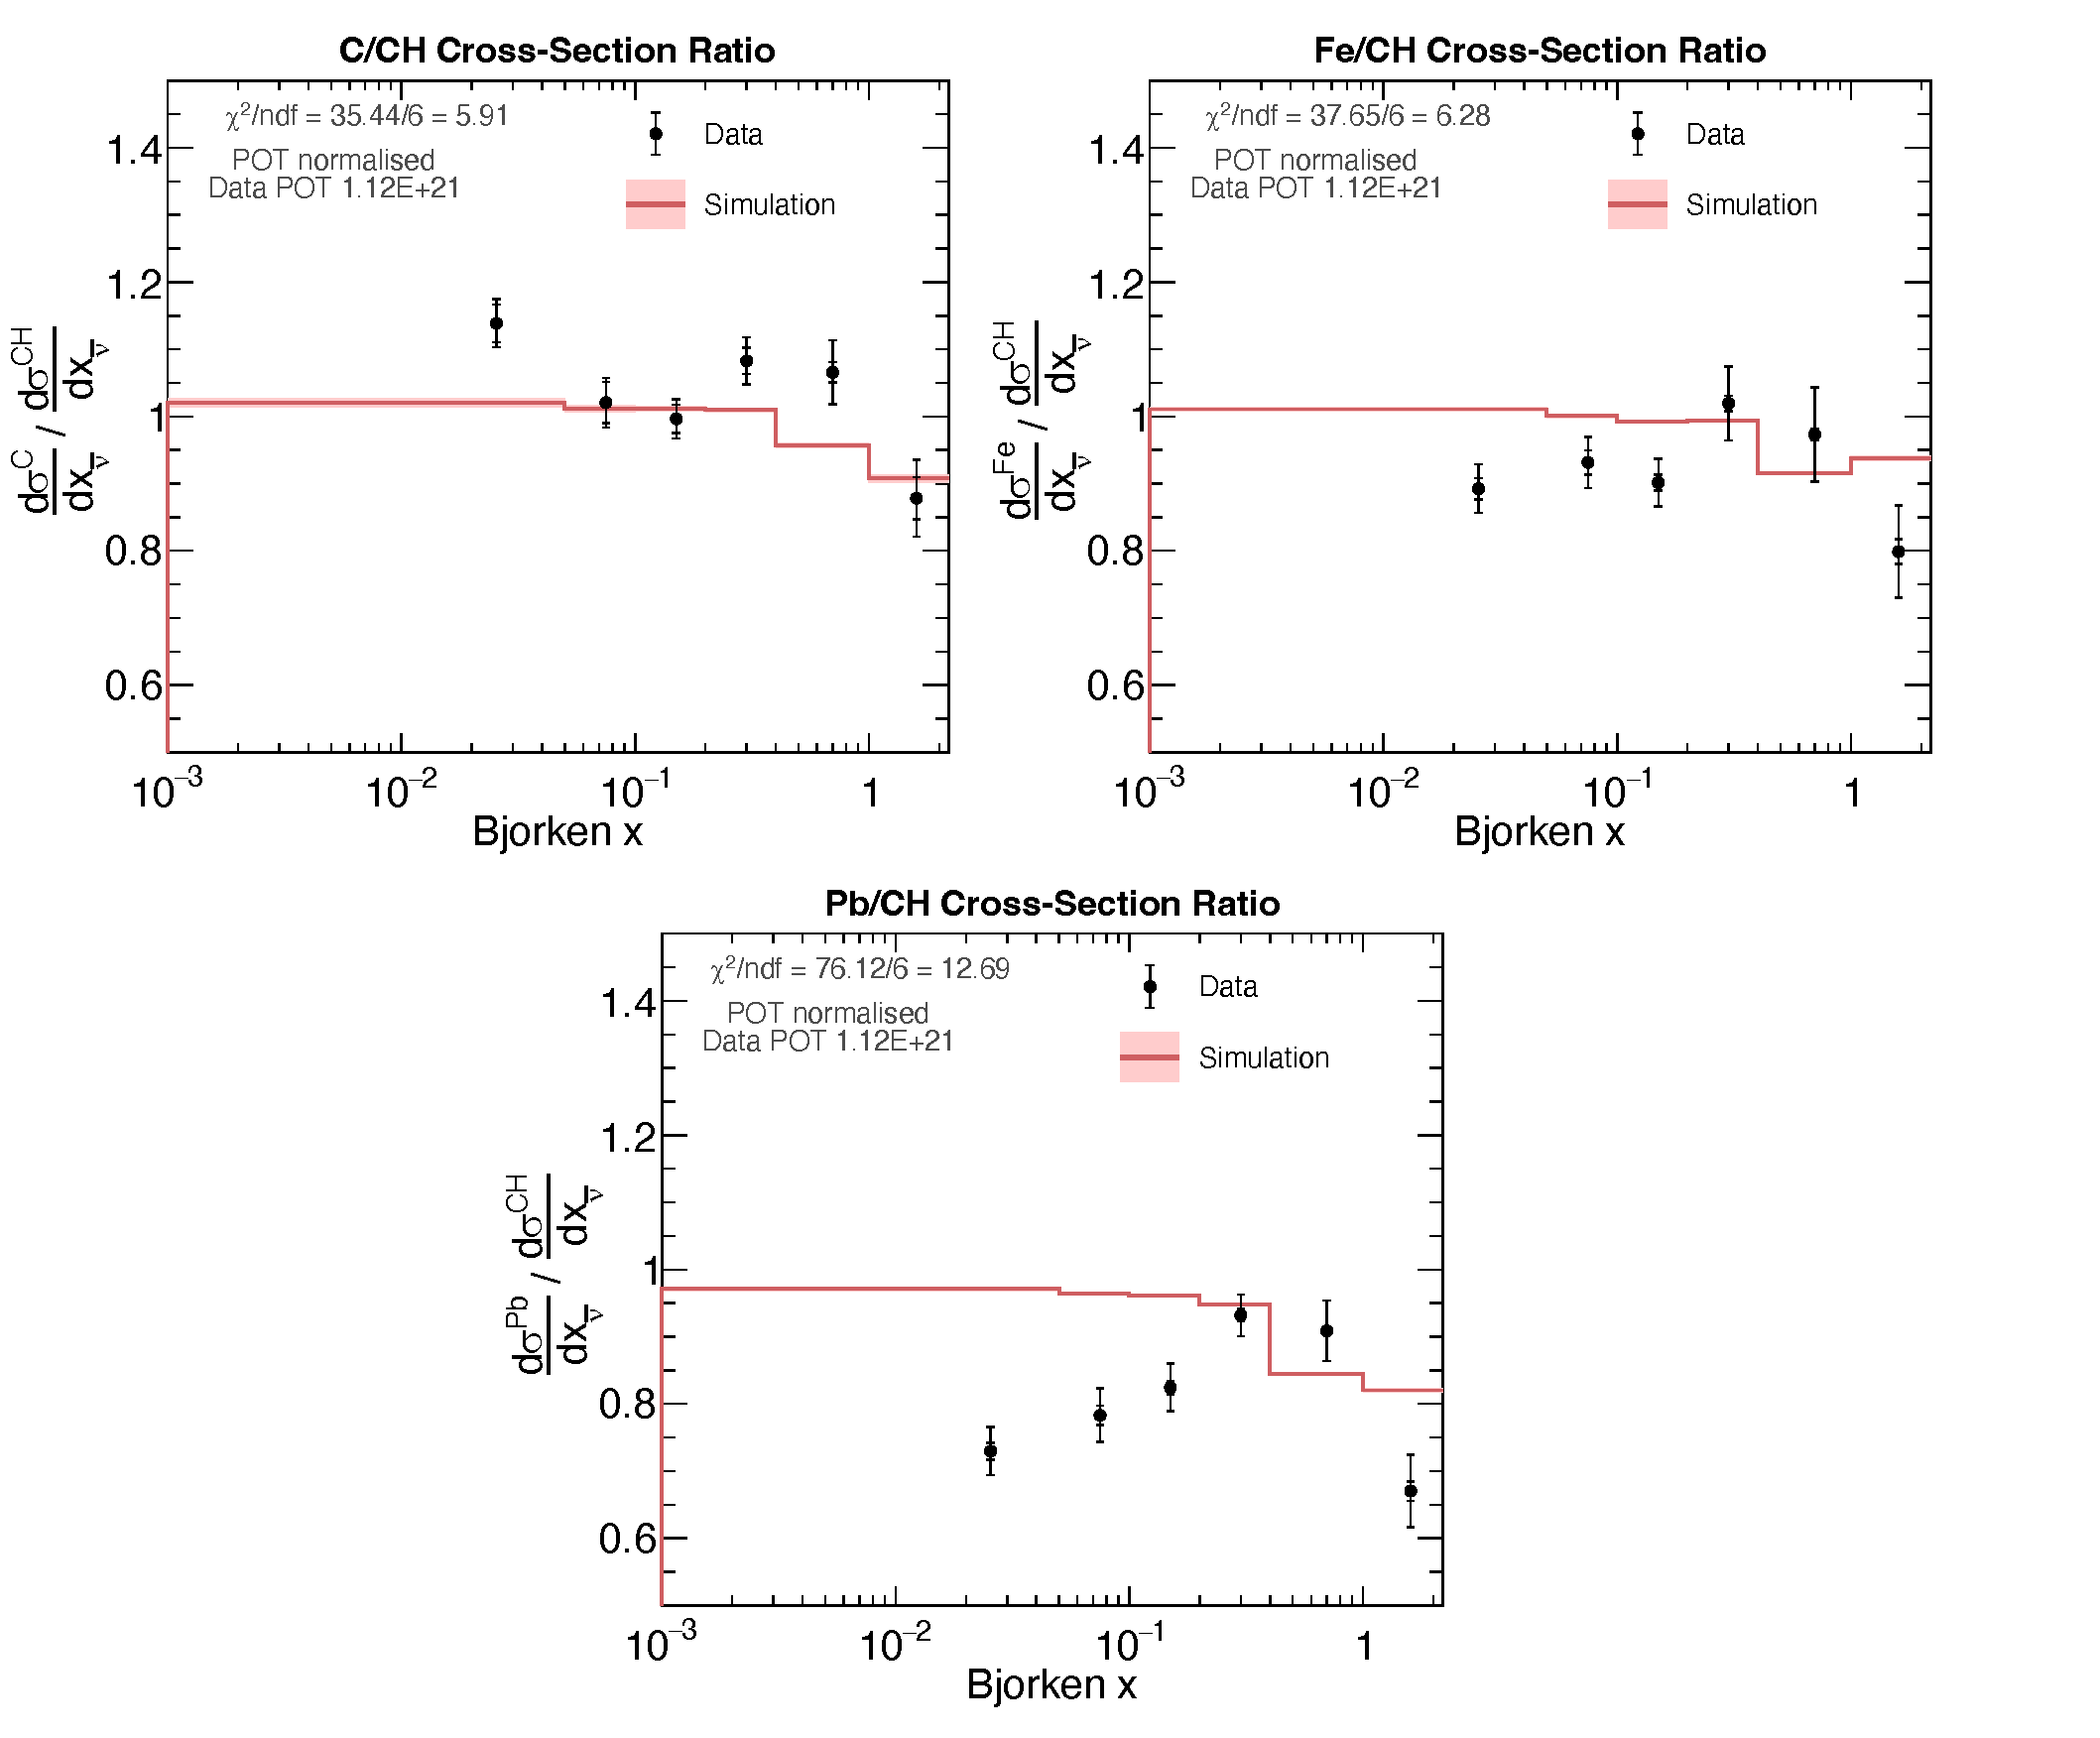
\includegraphics[width=1.\textwidth]{09results/figures/ratios_x.pdf}}%
    \caption{Carbon-to-scintillator (top left), iron-to-scintillator (top right), and lead-to-scintillator (bottom) cross-section ratios in Bjorken $x$. The data points carry both statistical (inner error bar) and systematic (outer error bar, which is the sum of statistical and systematic errors) uncertainties. The error band around the simulation predictions represents its statistical error. Note the $A$-dependent difference across the measured ratios, particularly in the low-Bjorken $x$ region.}
    \label{fig:ratio_x}
\end{figure}

The cross-section ratios for iron and lead in Bjorken $x$ in Figure~\ref{fig:ratio_x} exhibit significant disagreement with the underlying simulation in the low $x$ region. These ratios particularly demonstrate a notable suppression of the iron and lead cross-section in this region compared to the scintillator, and the suppression grows with the size of the nucleus. This is in agreement with MINERvA's first investigation of such effects in the low-energy inclusive neutrino scattering~\cite{Tice_PhysRevLett.112.231801}. Note that the results of this analysis represent the first comprehensive and statistically significant investigation of such effects across various nuclei in the medium-energy inclusive antineutrino sample. The low-energy equivalent was not possible due to limited statistics. Compared to the neutrino results in low energy in Ref.~\cite{Tice_PhysRevLett.112.231801}, this analysis was performed using roughly 10$\times$ more interactions in each nucleus.

The depletion in the cross-sections for heavy targets at low $x$, referred to as shadowing-like region, mainly due to the DIS contribution is generally expected, and it is attributed to the destructive interference of hadronic fluctuations of the intermediate boson that multiple-scatter off surface nucleons,~\cite{KOPELIOVICH2013314, BEBCWA59:1989nmi, Tice_PhysRevLett.112.231801}, as explained in Chapter~\ref{ch:measurement}. There are several reasons why the depletion may be larger in the data than predicted by the simulation. First, the shadowing corrections included in the simulation prediction are based on charged lepton data, which, unlike antineutrinos, do not have axial-vector contributions. Additionally, the same shadowing corrections based on iron data are also applied to carbon and lead \cite{BODEK2005113}, as mentioned in Chapter~\ref{ch:dataAsimulation}. Furthermore, more than 85\% of the data has $Q^2 < $ 1 (GeV/$c$)$^2$, whereas the underlying simulation is tuned to the perturbative region of higher $Q^2$ data.
%\enlargethispage{1\baselineskip}


Importantly, interpreting the observed suppression of heavy target cross-sections at low $x$ is challenging, as it is impossible to disentangle FSI and nuclear effects due to the inclusive nature of the analysis. FSI effects may distort the observed Bjorken $x$ distribution by increasing or decreasing the observed recoil energy, with such effects possibly more pronounced in heavier nuclei, introducing strong nuclear dependence effects. Additional complexity also arises due to the interplay between pion production and deep inelastic scattering in the low $x$ region, which may be resolved with MINERvA's incoming deep and shallow inelastic scattering results. 

The high-$x$ region, dominated by quasi-elastic scattering across various nuclei, is also overpredicted in the cross-section ratios for iron and lead. However, its interpretation is also somewhat complex. The corresponding migration matrices in Section~\ref{sec:migration_unfolding} showed large smearing in this region, and while the model dependence in unfolding was studied, the quasi-elastic scattering in antineutrino interactions results in neutrons, which are often invisible to the calorimetric recoil reconstruction. The correction to the recoil energy accounting for this is inherently model-dependent as described in Chapter~\ref{ch:Reconstruction}.

\begin{figure}[t!] 
    \centering
    {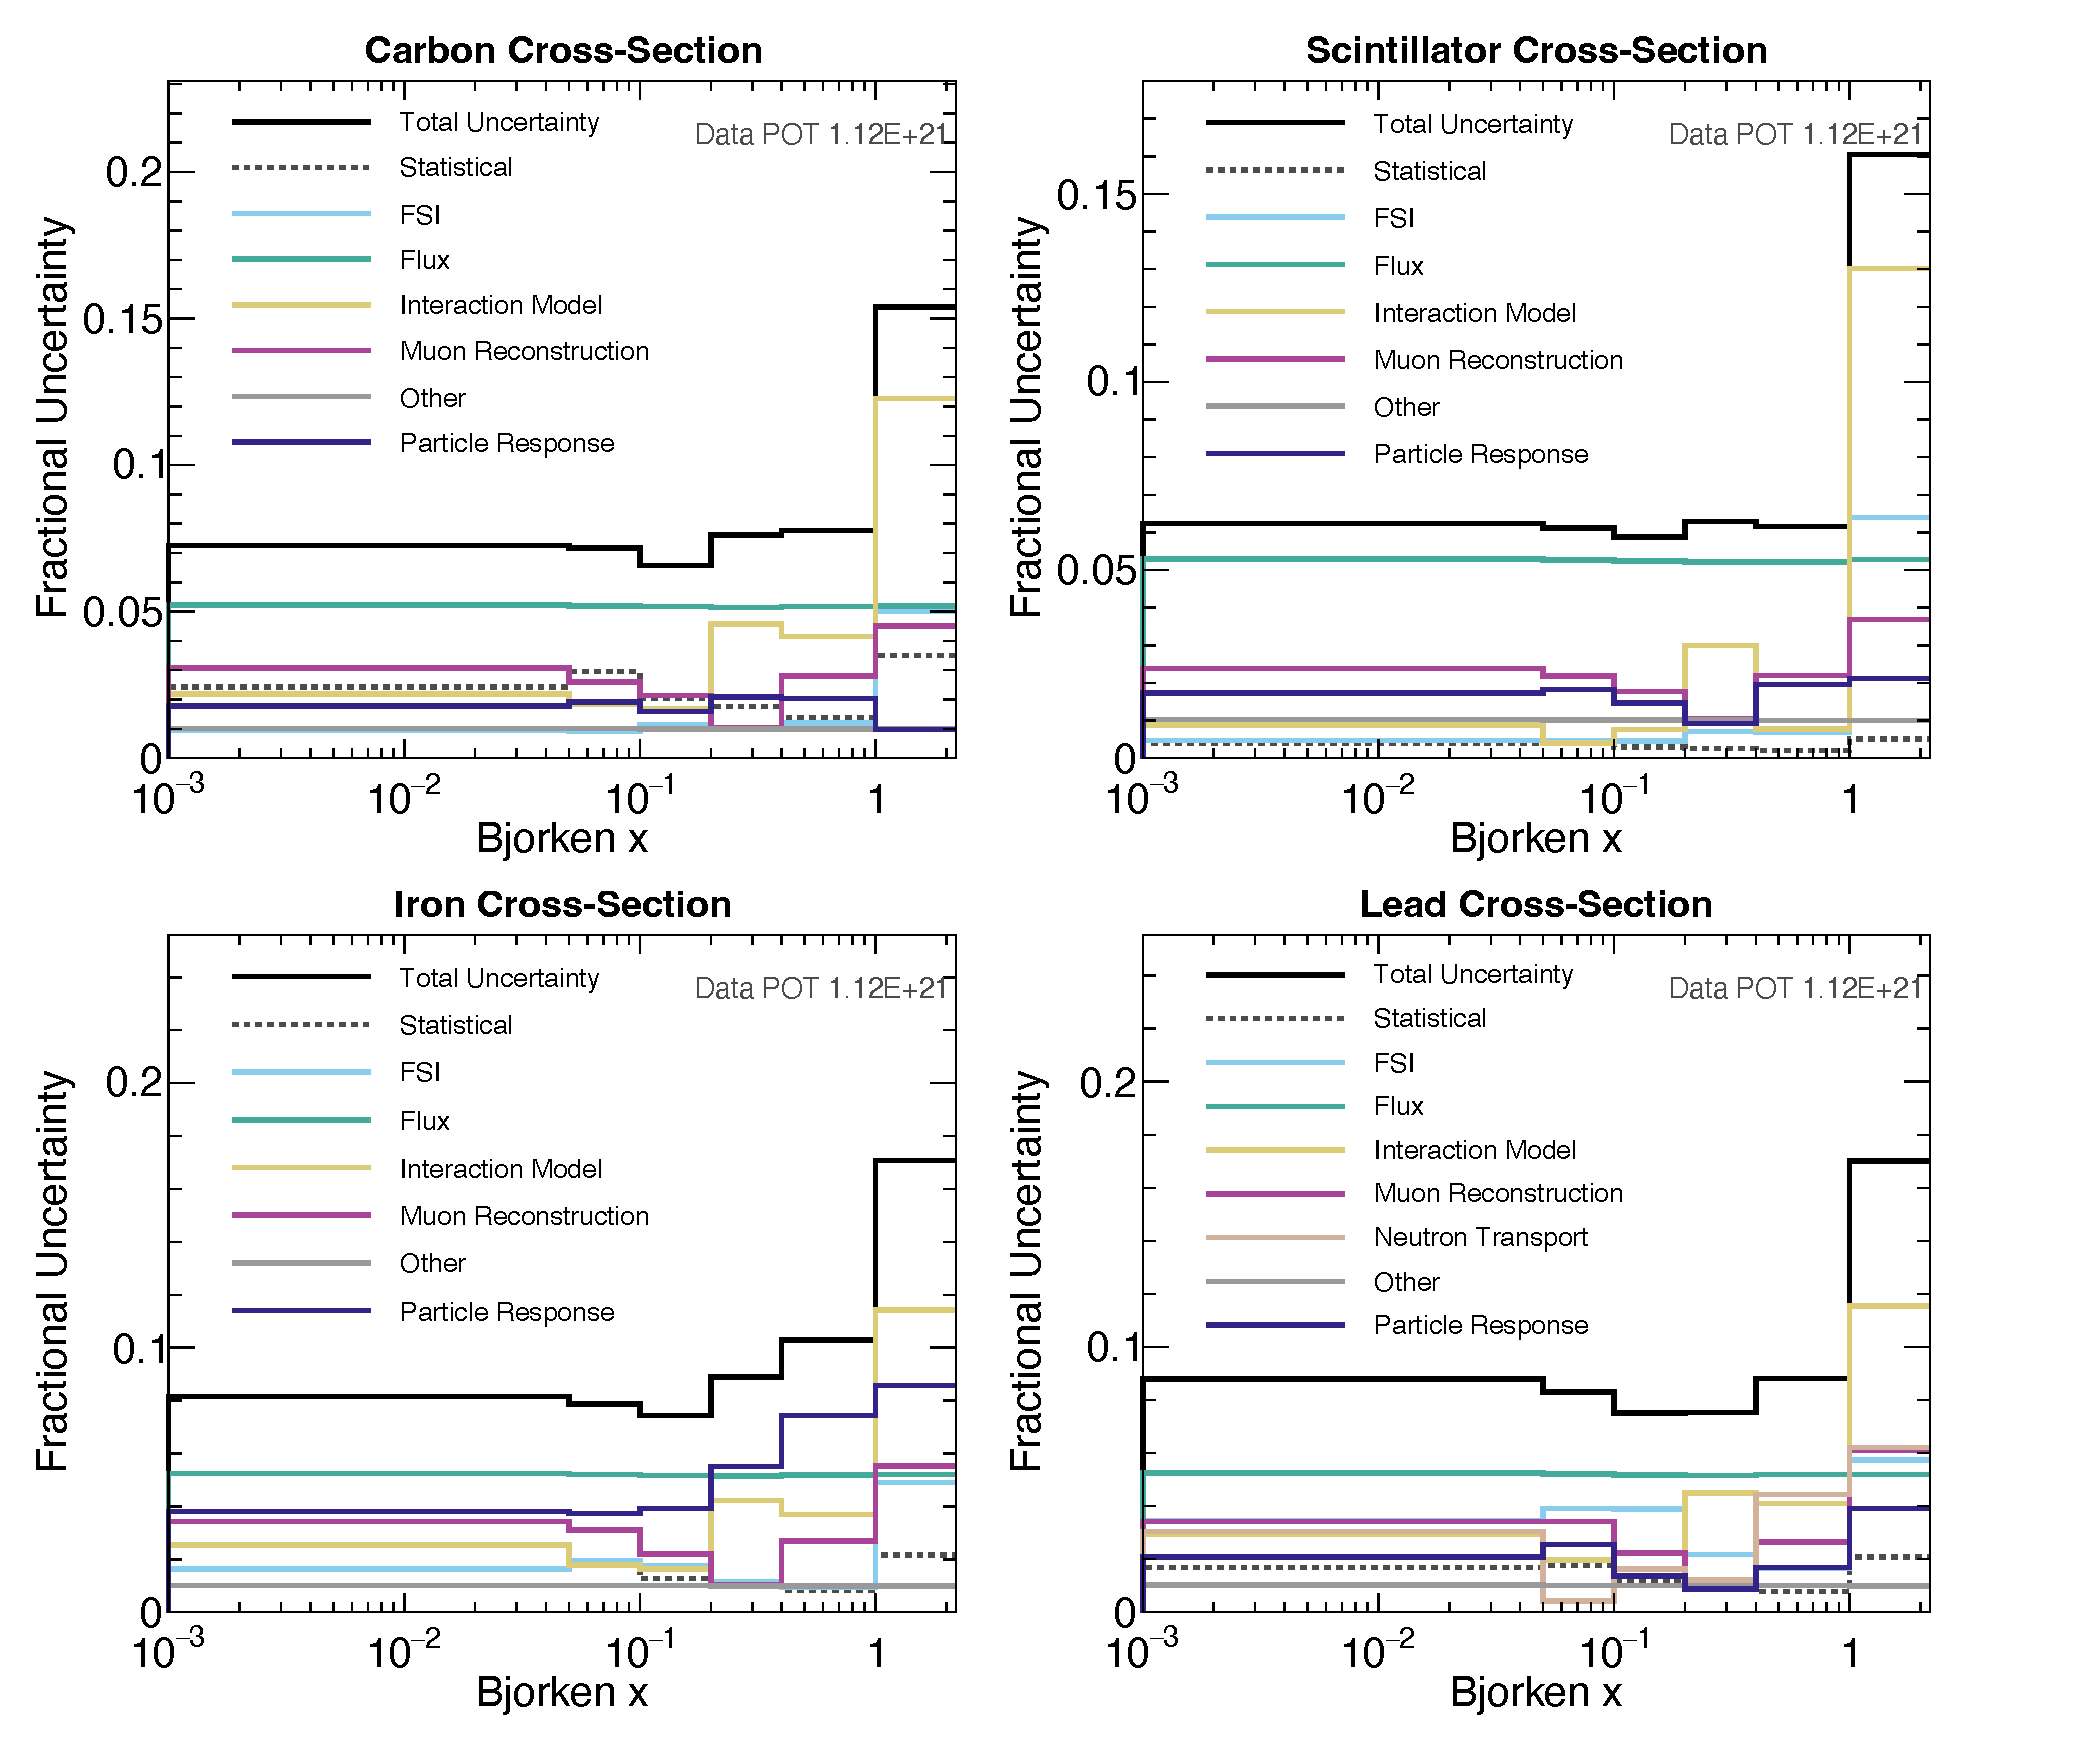
\includegraphics[width=1.\textwidth]{09results/figures/xsec_x_fracErr.pdf}}%
    \caption{Breakdown of the fractional uncertainties on the data cross-section in Bjorken~$x$ for carbon, hydrocarbon, iron, and lead (from left to right, top to bottom). Note that, in general, the cross-sections are dominated by uncertainties on flux, with the exception of the high-$x$ region, which is dominated by uncertainties on the underlying interaction model.}
    \label{fig:xsec_x_fracErr}
\end{figure}

Furthermore, the $x > 1$ region simulated by GENIE comes mostly from smearing from final-state interactions and does not include predictions of interactions from short-range correlated nucleons. These are expected to occur in this region based on electron-scattering data~\cite{CLAS:PhysRevLett.96.082501, SRC:annurev}. Also, the exploratory study of the potential bias due to neutron modelling corrections in Section~\ref{sec:migration_unfolding} suggested a need for additional uncertainty in this region, as discussed in Chapter~\ref{ch:systematics}. Nevertheless, this analysis presents the first attempt to measure this region in antineutrino scattering and the data seems to indicate the need for a larger suppression at high $x$ compared to carbon. However, the challenges described above preclude the analysis from making any definitive conclusions. 

\begin{figure}[t!] 
    \centering
    {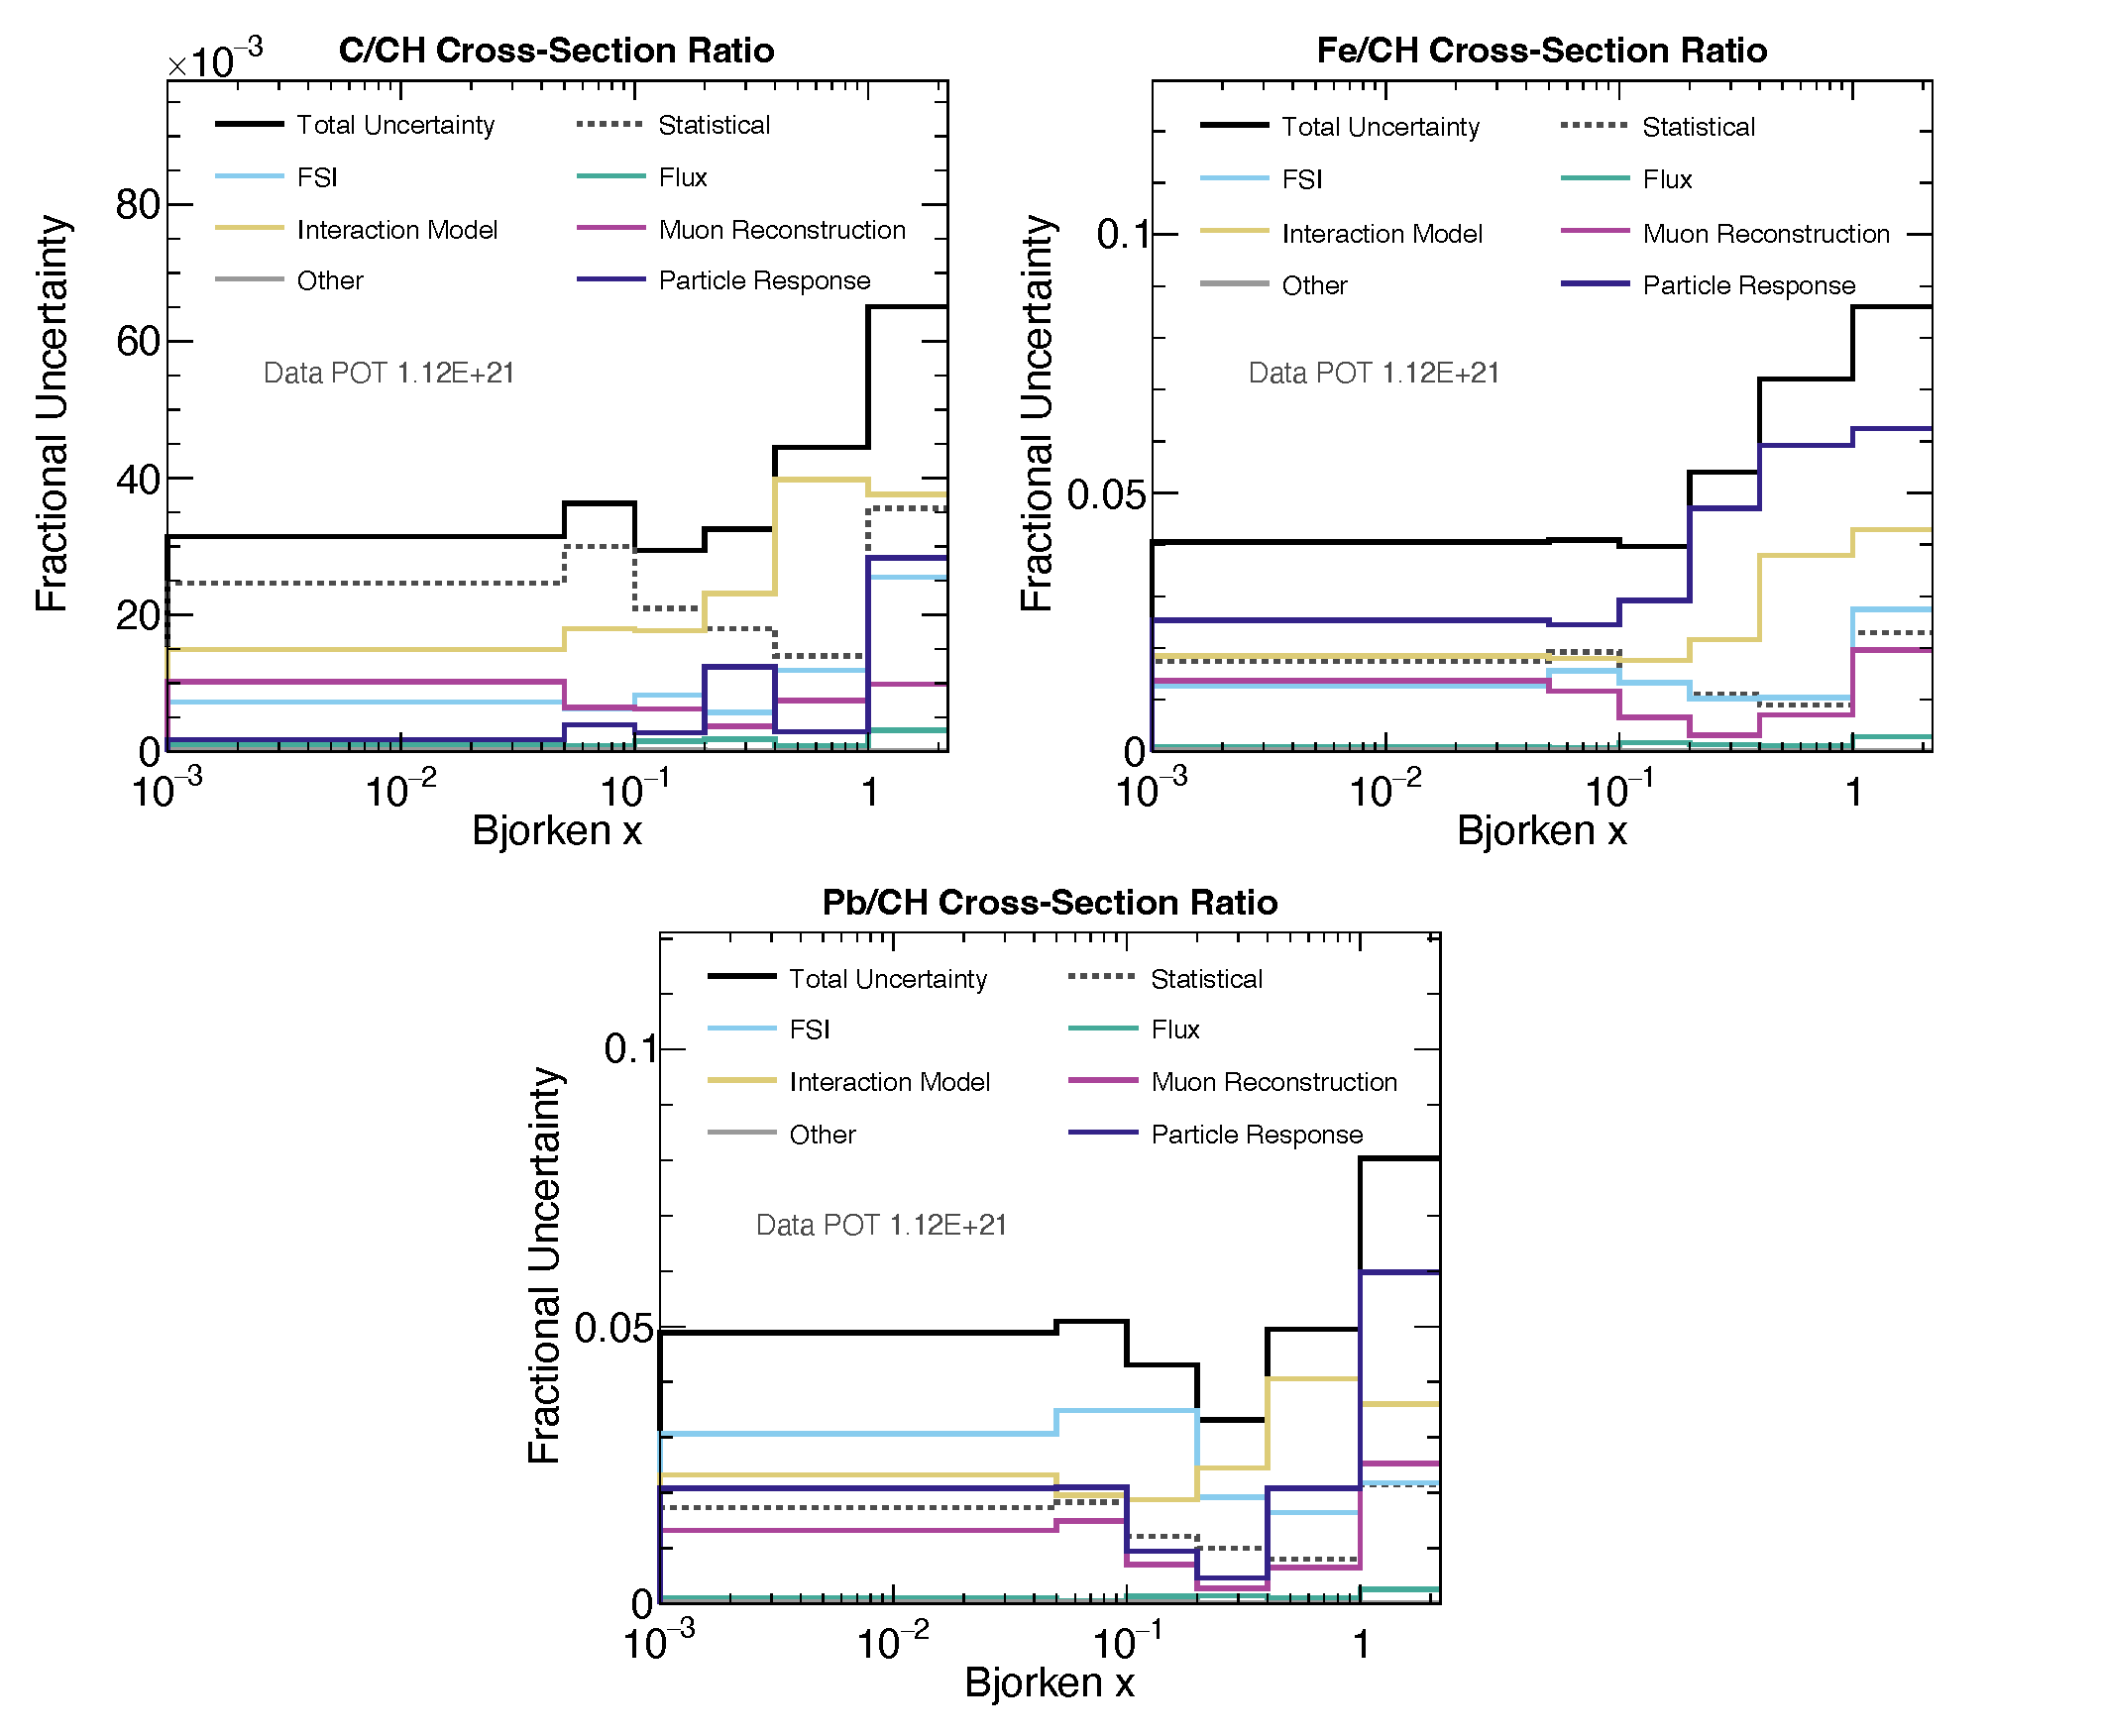
\includegraphics[width=1.\textwidth]{09results/figures/ratios_x_fracErr.pdf}}%
    \caption{Breakdown of the fractional uncertainties on the data cross-section ratios to scintillator for carbon (top left), iron (top right), and lead (bottom) in Bjorken~$x$. Note that the flux and detector-related uncertainties are mostly cancelled out.}
    \label{fig:ratio_x_fracErr}
\end{figure}

Similarly to $p_{\text{T}}$, the carbon-to-scintillator ratio is most consistent with the simulation and with unity. The sideband effects discussed above for $p_{\text{T}}$ could potentially explain the differences from the underlying prediction of the ratio. Moreover, the low-$x$ region is also sensitive to the recoil energy scale, prompting a potential investigation into whether the recoil scale differs between the nuclear target region and the scintillator tracker.


Figures~\ref{fig:xsec_x_fracErr} and \ref{fig:ratio_x_fracErr} summarise the breakdowns of the fractional uncertainties on the Bjorken $x$ cross-sections and the cross-section ratios for various nuclei. Similar to the~$p_{\text{T}}$ cross-section, the Bjorken $x$ cross-section is dominated by flux uncertainty. The $x > 1$ region is governed by the understanding of the underlying interactions, i.e. `Interaction Model' error band, for the reasons described above. The C/CH ratio is mostly limited by the underlying statistics (except at large $x$). 

Overall, in all ratios, the `Interaction Model' error band represents the leading source of systematic uncertainty. Akin to the $p_{\text{T}}$ results, the contribution in iron from the `Particle Response' uncertainty band, i.e. GEANT4 neutron modelling, is being investigated. However, the `Particle Response' in this case also includes the calorimetric detector response, as Bjorken $x$ depends on recoil reconstruction, making its contribution overall larger than in $p_{\text{T}}$. Finally, the `FSI' uncertainty becomes more prominent in the ratio as the nucleus in the numerator gets heavier. %Similar to the $p_{\text{T}}$ cross-section results, the full covariance matrices for the measured Bjorken $x$ cross-sections are included in Appendix~\ref{ch:appendix_covarianceMatrices}.


\section{Model comparisons}


It is important to review the measured results in the context of other (anti)neutrino event generators that implement different interaction models than the underlying simulation used in the analysis. The different generator-to-data comparisons might give some insight into various aspects of the models, especially when extended to larger $A$, inform the neutrino interaction community, and potentially lead to further developments. Both the cross-sections and cross-section ratios are compared with a newer version of \mbox{GENIE~\cite{genie_ANDREOPOULOS201087,genie_andreopoulos2015}}, and a different event generator called NEUT~\cite{Hayato:2009zz, HayatoPickering2021}, which is primarily used in (anti)neutrino oscillation analyses at the T2K experiment~\cite{t2k_ABE2011106}.

Various aspects of the different generators that are relevant to the analysis and in which they differ from the underlying simulation (outlined in Chapter~\ref{ch:dataAsimulation}) are briefly described below.

\vspace{5pt}
% https://genie-docdb.pp.rl.ac.uk/DocDB/0000/000002/003/man.pdf
\noindent \textbf{GENIE version 3.0.6} \cite{genie3}: The resonant pion production is simulated by the Berger-Sehgal model~\cite{PhysRevD.76.113004} instead of the Rein-Sehgal\cite{REIN198179}. The Berger-Sehgal update includes effects due to the muon mass in the cross-section calculation~\cite{kuzmin, coherentMass_REIN2007207,Adler_2006}, and new implementation \cite{Nowak_2009} of different axial and vector form factors~\cite{PhysRevD.77.053001}. The parameters of the vector form factor are determined from electron scattering data \cite{PhysRevD.74.014009}. Furthermore, the FSI model is improved by emphasizing medium correlations between nucleons which suppress multiple scattering and have a strong $A$-dependence~\cite{genie3, PhysRevD.104.053006}.~There are two FSI models available, effective cascade $hA$ and full intranuclear cascade model $hN$. In addition, the differences between the individual labels in the model comparisons are:
% pion pole term which reproduce the expected Adler-screening effect at low $Q^2$ (because of the muon mass)
% diffractive model Rein and hyperon production using the pais model
% coherent pion production simulated by berger-seghal too
% used new implementation of axial and vector form factors based on Rarita-Schwinger 
% GENIE3 narrative
% https://indico.cern.ch/event/1175720/attachments/2470263/4237838/Resonances-20220627.pdf

\begin{itemize}
    \item GENIE3 G18\_02a/b uses the empirical 2p2h model \cite{genie_ANDREOPOULOS201087,katori2013meson}. The `a/b' tag represents the $hA$ and $hN$ FSI model, respectively. The label is a shorthand for the official GENIE 3 release G18\_02a/b\_02\_11a. 
    \item GENIE3 G18\_10a/b employs the local Fermi gas nuclear model \cite{RPANieves2004_PhysRevC.70.055503} instead of the relativistic Fermi gas \cite{RFG_SMITH1972605, 1975547}, and the quasi-elastic and 2p2h interactions are based on the Valencia model \cite{2p2hNieves2011_PhysRevC.83.045501}. Again `a' refers to $hA$ and `b' to $hN$ FSI model. The label is a shorthand for the official GENIE 3 release G18\_10a/b\_02\_11a. 
\end{itemize}

\vspace{5pt}
\noindent 
\textbf{NEUT version 5.4.1} \cite{Hayato:2009zz, HayatoPickering2021}: The resonant pion production is
simulated by the Berger-Sehgal~\cite{PhysRevD.76.113004}. A custom multi-pion-production model is used for $W < 2$ GeV$/c^2$, while deep inelastic scattering with $W > 2$ GeV$/c^2$ is simulated using PYTHIA/JETSET~\cite{Pythia_Sjostrand_2001}. Both are based on the Bodek-Yang model\cite{BodekYang_2003,BODEK2005113} parton distribution functions. The 2p2h interaction is simulated using the Valencia model \cite{2p2hNieves2011_PhysRevC.83.045501}. FSI uses a custom intranuclear cascade model. The two different labels have further distinguishing features:
%- developed for (anti)neutrino interactions on carbon and water, mostly for measurements of lepton kinematics
%- coherent Berger-Sehgal
%- diffractive Rein model
\begin{itemize}
    \item NEUT LFG ma105 uses the local Fermi gas nuclear model \cite{RPANieves2004_PhysRevC.70.055503} and the quasi-elastic scattering is based on the Valencia model \cite{2p2hNieves2011_PhysRevC.83.045501, Bourguille_2021} with $M_{A} = 1.05$ GeV$/c^2$.
    \item NEUT SF ma103 utilises the spectral function for the nuclear ground state with the associated quasi-elastic scattering \cite{Benhar:1994hw, Juszczak_2006, Furmanski:2015knr} with $M_{A} = 1.03$ GeV$/c^2$.
\end{itemize}
% what does it do for lead?
\noindent Note that the general differences between the various theoretical models were addressed in Chapter~\ref{ch:theory}.

% chi-squared statistic with general covariance matrix
In addition to the visual comparison, the agreement between the measured data and the various models is calculated using $\chi^2$, which takes into account bin-to-bin correlations,
\begin{equation}
    \chi^2 = \sum_{ij} (x_i - \mu_i) \text{cov}_{ij}^{-1} (x_j - \mu_j) \hspace{2pt} .
    \label{eq:fullyCorrelatedChi2}
\end{equation}
The $\text{cov}_{ij}$ represents the element of the covariance matrix defined in Chapter~\ref{ch:systematics}, $x_i$ is the data in bin $i$, and $\mu_i$ is the corresponding model prediction. Note that the $\chi^2$ differences in the inclusive sample are often small as some model changes do not have large impact on the inclusive cross-section.

Figures~\ref{fig:xsec_pT_modelComparison} and \ref{fig:ratio_pT_modelComparison} show the $p_{\text{T}}$ cross-section and cross-section ratio model comparisons, respectively, across the different nuclei. The corresponding fully-correlated $\chi^2$s per degree of freedom (the number of bins) are summarised in Tables~\ref{table:xsec_modelComparison_pT} and~\ref{table:xsecRatio_modelComparison_pT}.
The Bjorken $x$ results are compared to other models in Figures \ref{fig:xsec_x_modelComparison} and \ref{fig:ratio_x_modelComparison} with the corresponding $\chi^2$s presented in Tables~\ref{table:xsec_modelComparison_x} and~\ref{table:xsecRatio_modelComparison_x}, respectively.

\begin{figure}[t!] 
    \vspace{30pt}
    \centering
    {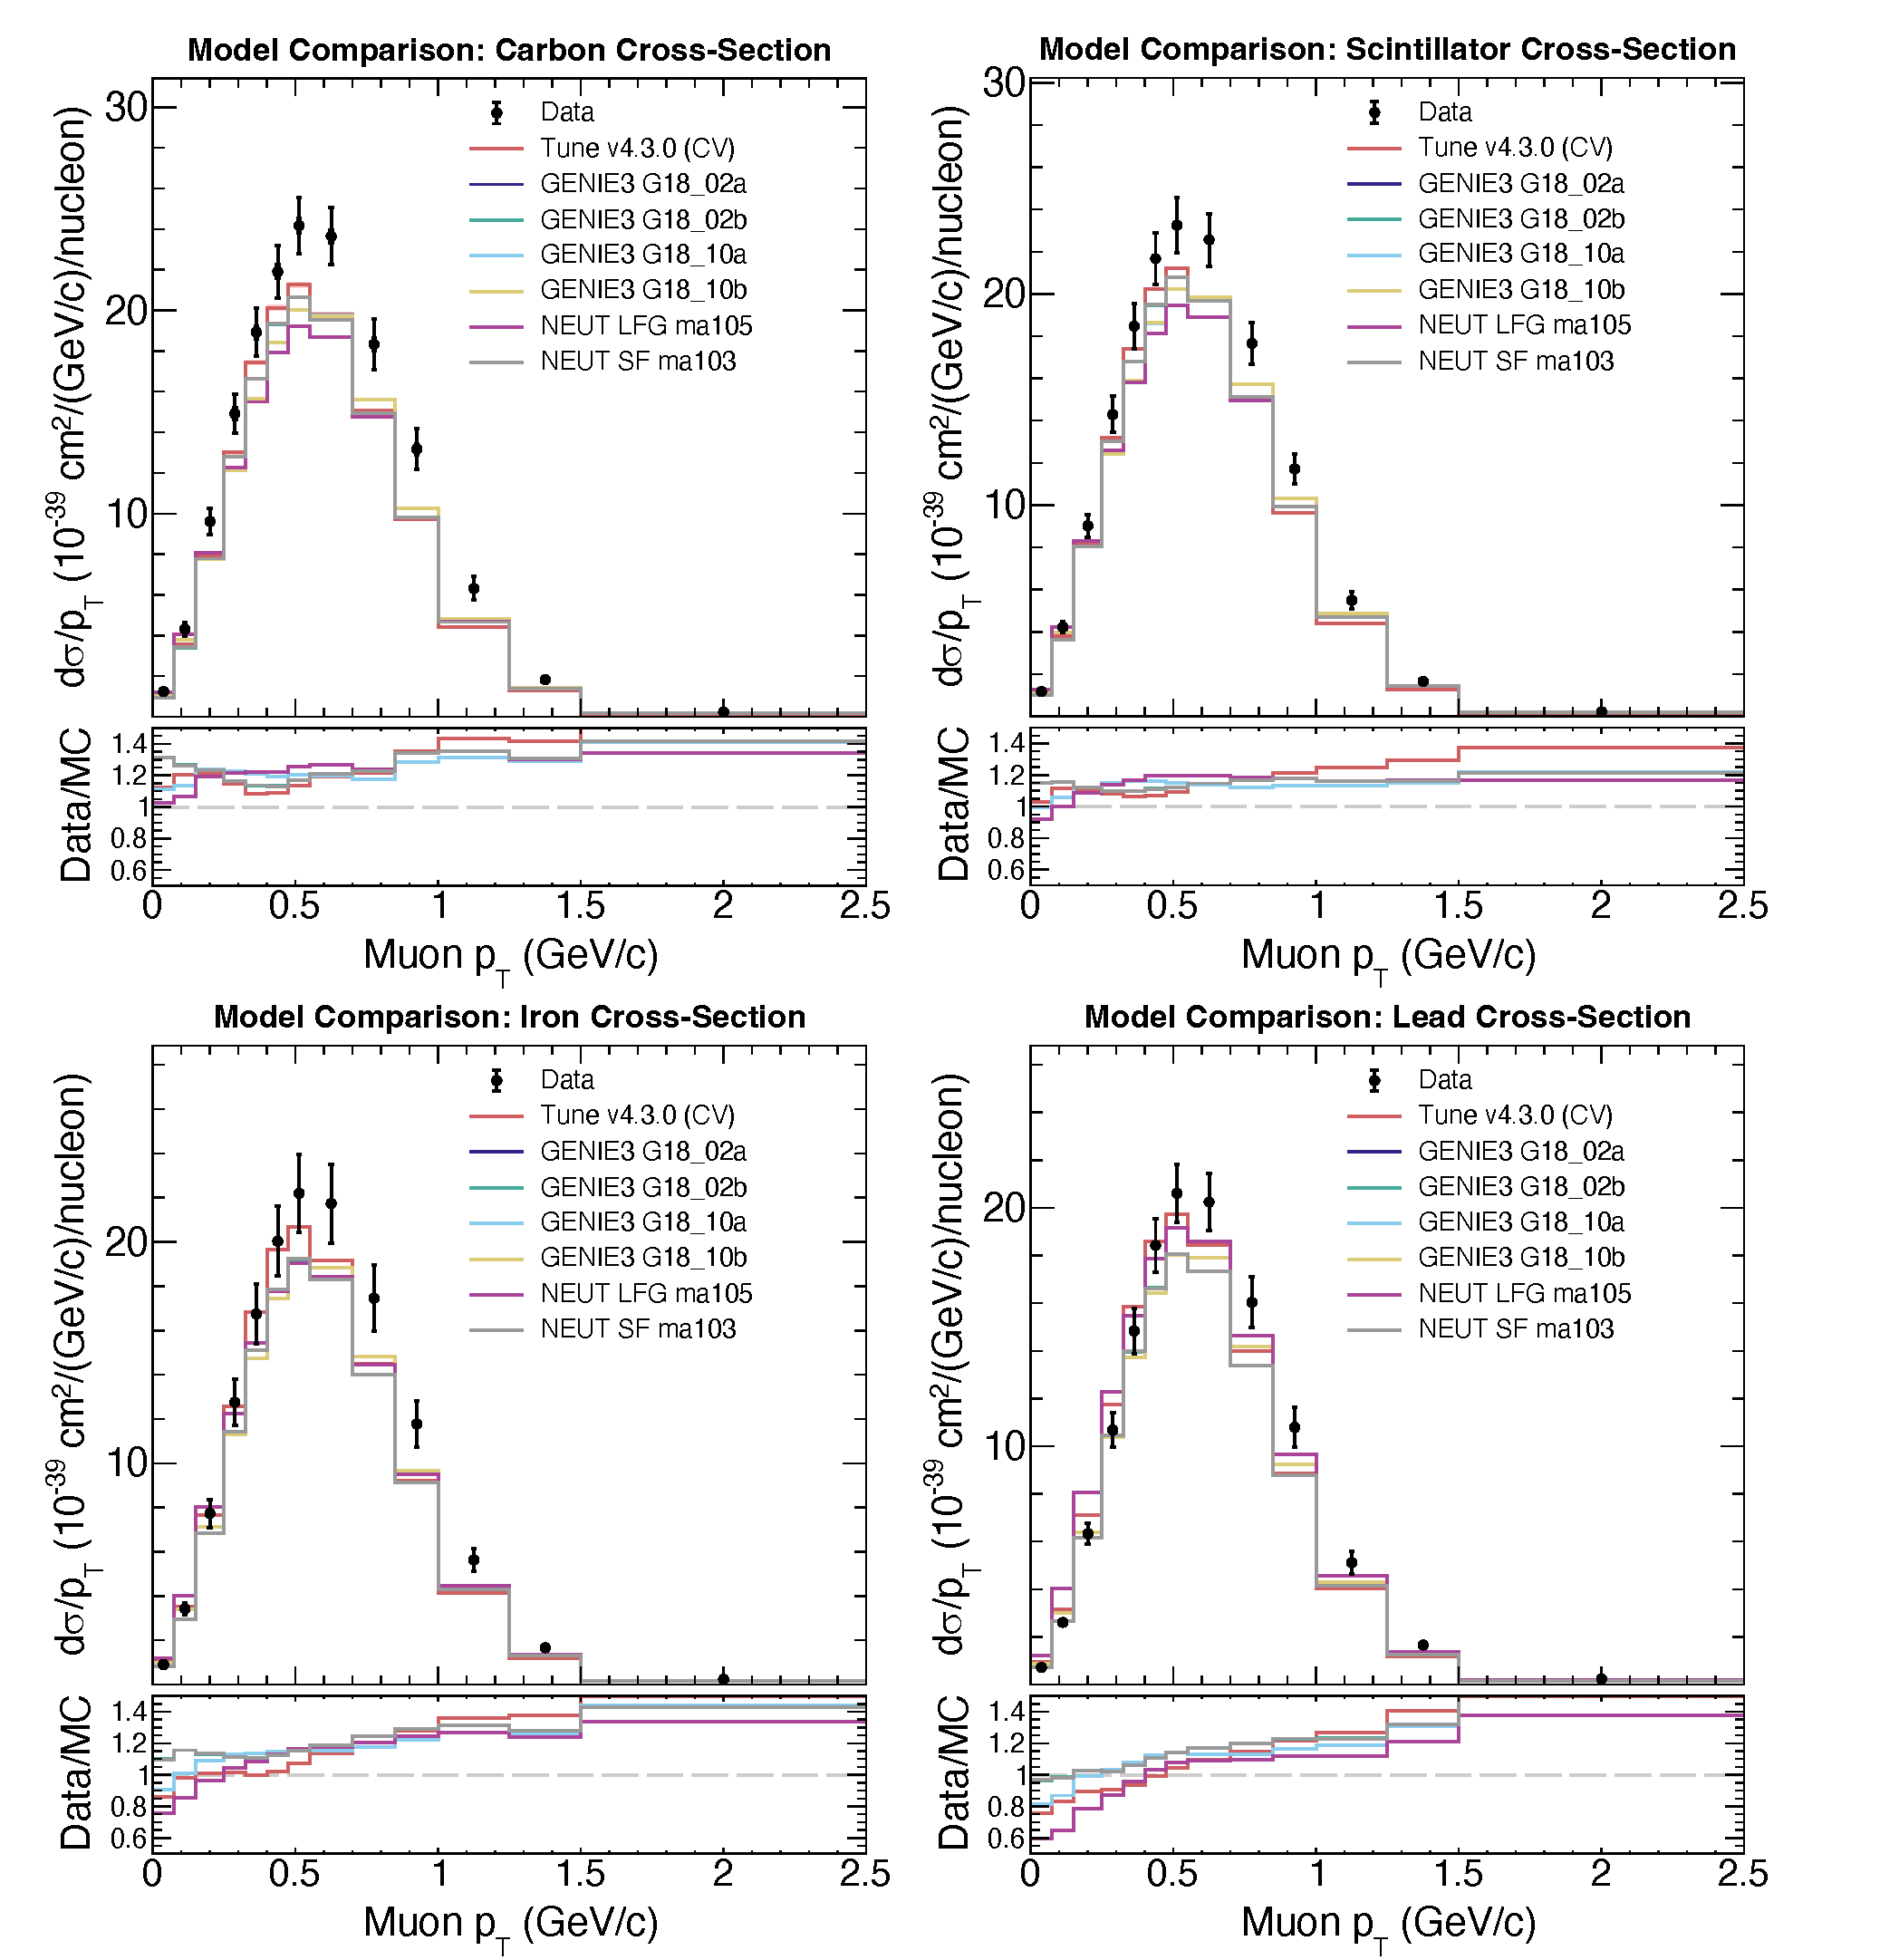
\includegraphics[width=1.\textwidth]{09results/figures/xsec_pT_modelComparison.pdf}}%
    \caption{Measured carbon, scintillator, iron, and lead (from left to right, top to bottom) cross-section as a function of antimuon $p_{\text{T}}$ compared to various antineutrino generator predictions. The inner error bar on the data indicates the statistical error while the outer error bar corresponds to the total, i.e. statistical + systematic, error. The statistical errors on the various model predictions are not shown for clarity (but they are also negligible). The bottom panel indicates the agreement between the data and various models through their respective data-to-model prediction ratios.}
    \label{fig:xsec_pT_modelComparison}
\end{figure}

\begin{figure}[t!] 
    \centering
    {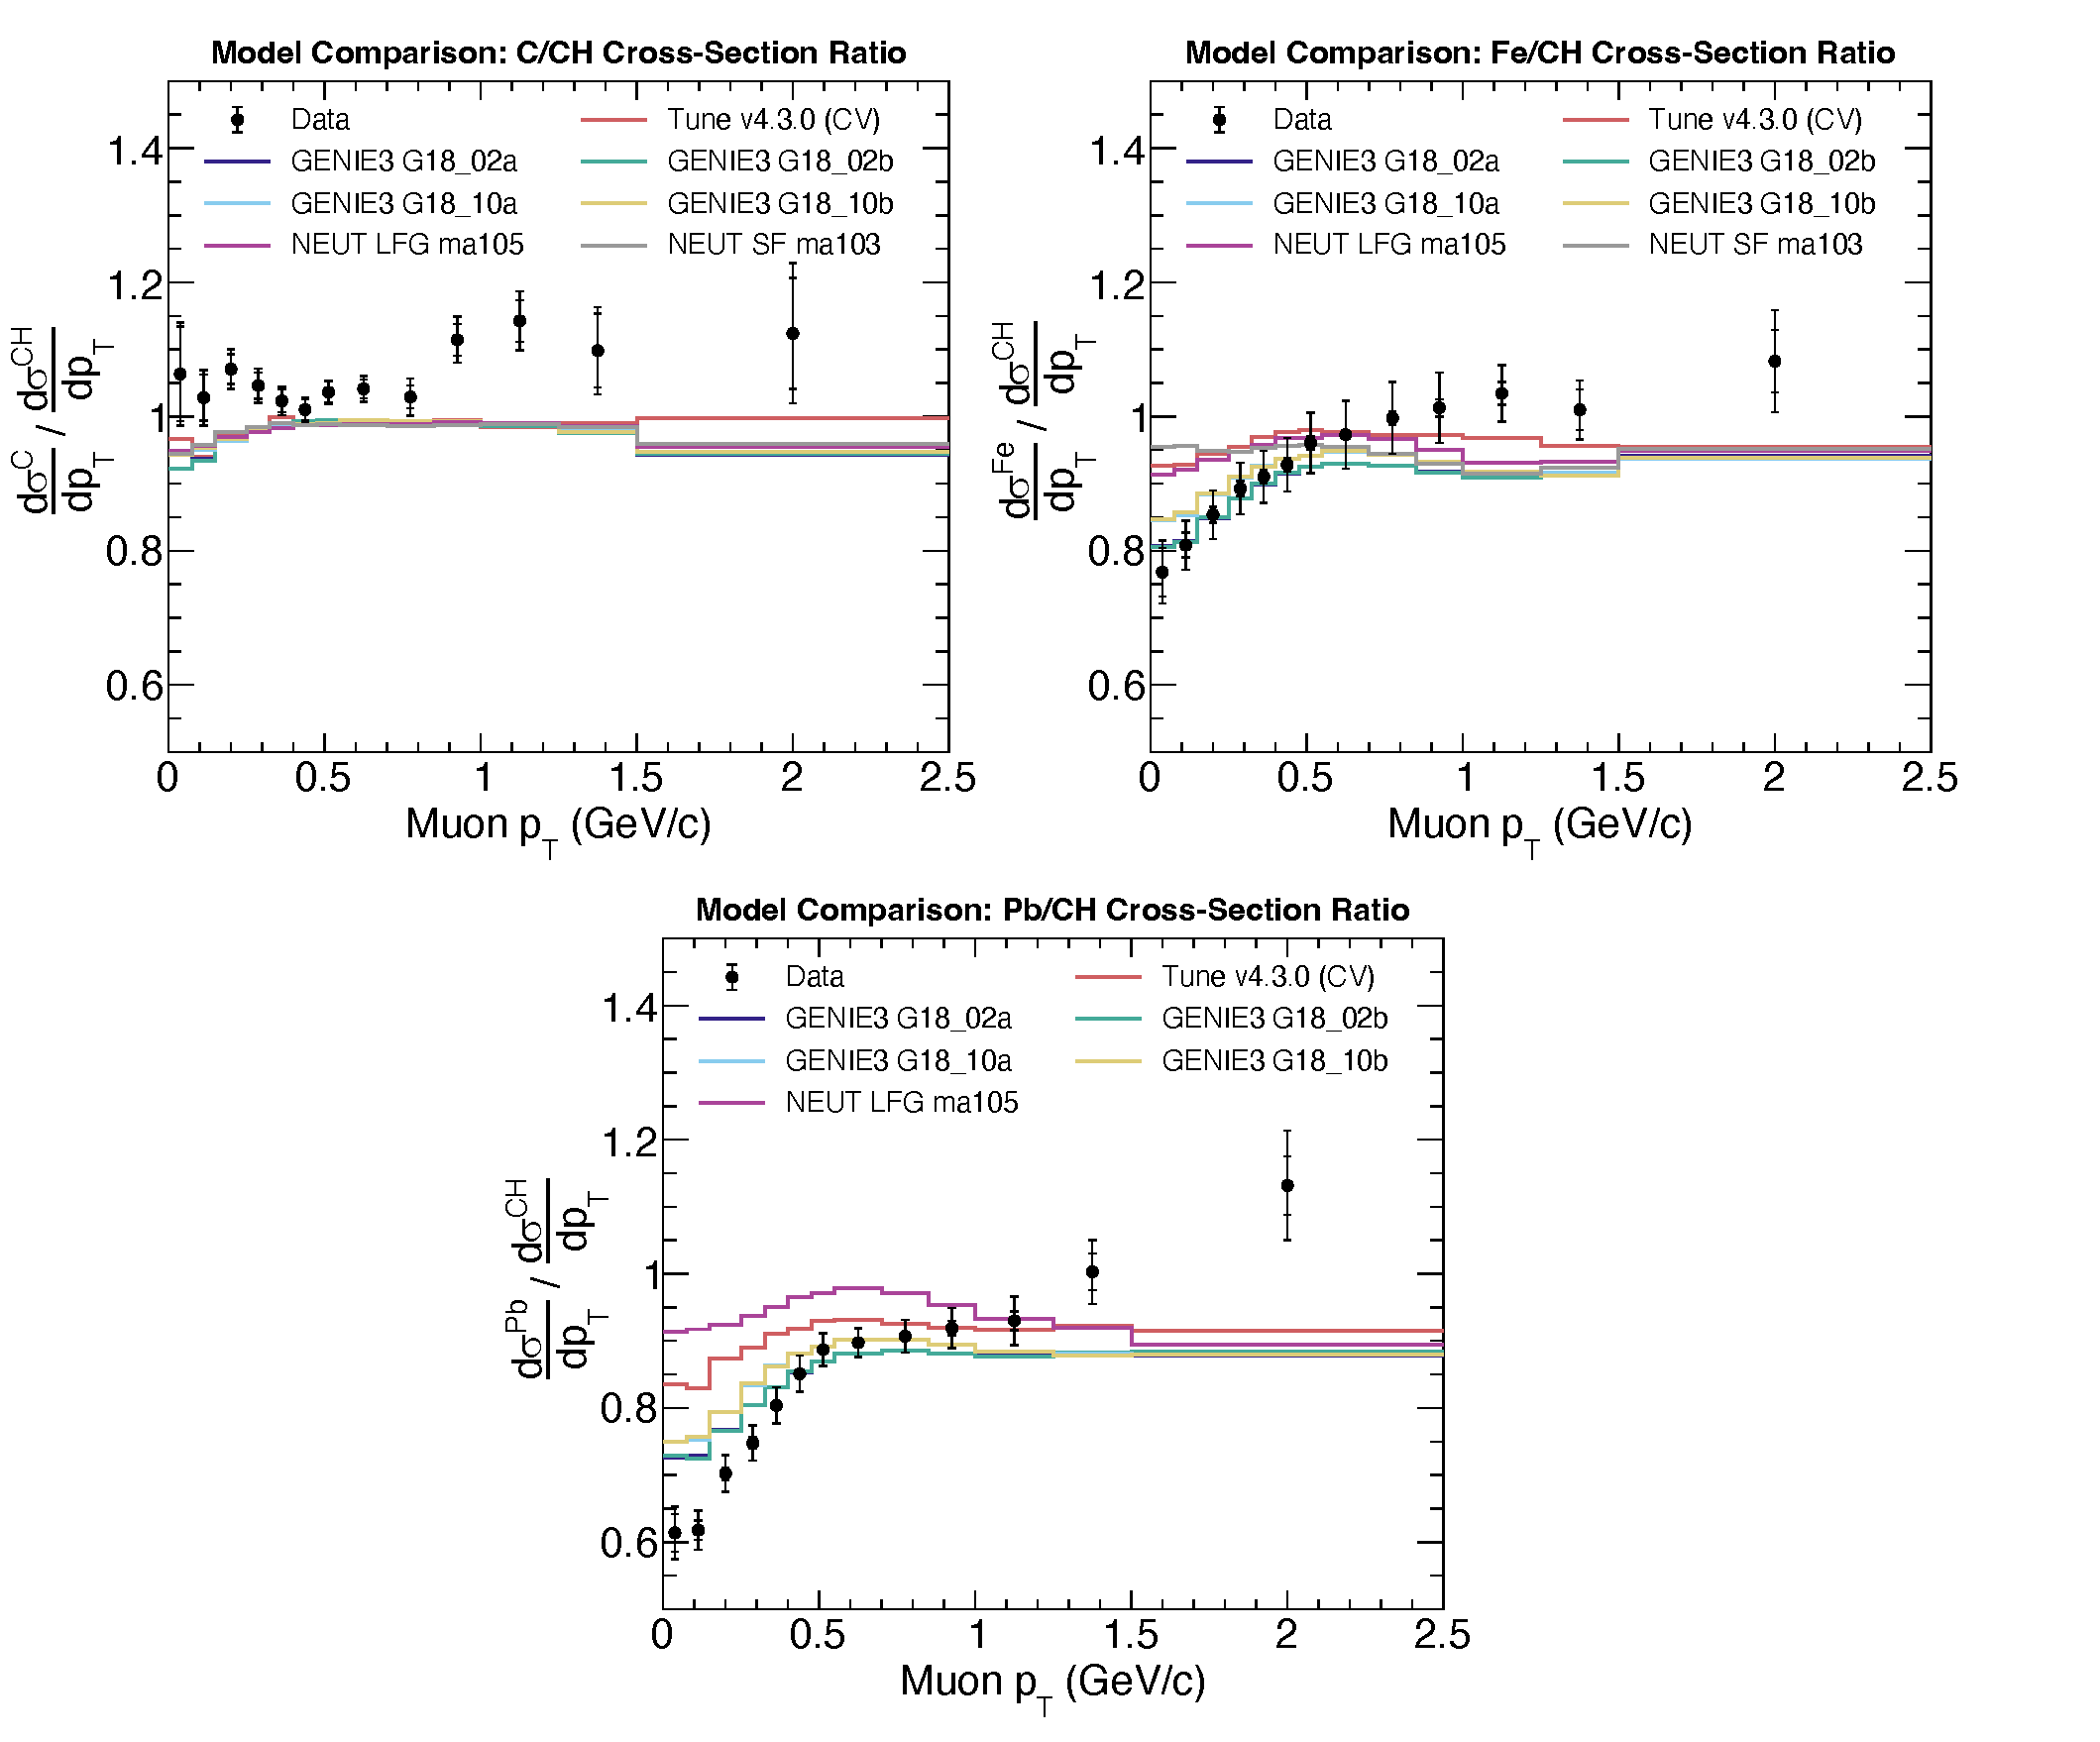
\includegraphics[width=1.\textwidth]{09results/figures/ratios_pT_modelComparison.pdf}}%
    \caption{Measured carbon-to-scintillator (top left), iron-to-scintillator (top right), and lead-to-scintillator (bottom) cross-section ratios in antimuon $p_{\text{T}}$ compared to various antineutrino generator predictions. The data is displayed with both the statistical (inner error bars) and the total (outer error bars) uncertainty. Note that the suppression predicted by the GENIE 3 models at low $p_{\text{T}}$ mostly follows the shape of the data.}
    \label{fig:ratio_pT_modelComparison}
\end{figure}


The $p_{\text{T}}$ cross-section data generally indicates a preference for the new version of GENIE 3, with a slight inclination towards G18\_02a/b. G18\_10a/b, on the other hand, tends to provide a slightly better prediction for the carbon data based on the calculated~$\chi^2$. The improvements over the underlying simulation are likely to stem mainly from better modelling of the low $p_{\text{T}}$ regions using updated axial and vector mass form factors. The NEUT model using the spectral function nuclear ground state performs similarly well for carbon, scintillator, and iron. Overall, the models tend to underpredict the data, except in the low $p_{\text{T}}$ region for heavier nuclei where the models overpredict. All models fail to reproduce the high $p_{T}$ behaviour.
% LFG versus RFG initial-state nucleon models is small because affects mostly CCQE in GENIE and not 2p2h or RES (and nos IDS)

\begin{table}[t!]
    \centering
    \begin{adjustbox}{width=1.01\textwidth,center=\textwidth}
    \begin{tabular}{c c c c c c c c}
    \hline \\ [-1.5 ex]
    \multirow[c]{2}{*}{Cross-section} & \multicolumn{7}{c}{Model $\chi^2$/ndf for $p_{\text{T}}$ (ndf = 13) } \\ [0.8ex]
    & CV & G18\_02a & G18\_02b & G18\_10a & G18\_10b & LFG\_ ma105 & SF\_ma103\\ [0.5ex] % inserts table %heading
    \hline
    \hline \\[-1.9ex]
    Carbon & 2.64 & 2.15 & 2.15 & 1.67 & 1.67 & 2.24 & 2.15 \\
    %\hline
    Scintillator & 10.35 & 4.37 & 4.47 & 12.77 & 12.22 & 40.75 & 4.37\\
    %\hline
    Iron & 3.04 & 1.63 & 1.67 & 3.12 & 3.13 & 9.60 &1.63 \\
    %\hline
    Lead & 6.22 & 3.20 & 3.11 & 9.07 & 9.24 & 39.59 & 3.20 \\

    \hline
    \end{tabular}
    \end{adjustbox}

    \caption{Fully correlated $\chi^2$/ndf calculated according to Equation~\ref{eq:fullyCorrelatedChi2} to assess the agreement between the measured data and the various models for carbon, scintillator, iron, and lead cross-section in antimuon $p_{\text{T}}$. Note that the relatively large $\chi^2$/ndf for the scintillator is attributed to the large statistics of the sample. The first numerical column indicates the agreement with the underlying simulation prediction.}
    \label{table:xsec_modelComparison_pT}
\end{table}


\begin{table}[t!]
    \vspace{20pt}
    \centering
    \begin{adjustbox}{width=1.01\textwidth,center=\textwidth}
    \begin{tabular}{c c c c c c c c}
    \hline \\ [-1.5 ex]
    \multirow[c]{2}{*}{Cross-section ratio} & \multicolumn{7}{c}{Model $\chi^2$/ndf for $p_{\text{T}}$ (ndf = 13) } \\ [0.8ex]
     & CV & G18\_02a & G18\_02b & G18\_10a & G18\_10b & LFG\_ ma105 & SF\_ma103\\ [0.5ex] % inserts table %heading
    \hline
    \hline \\[-1.9ex]
    C/CH & 4.93 & 5.72 & 5.75 & 5.80 & 5.74 & 5.90 & 5.60 \\
    %\hline
    Fe/CH & 2.35 & 1.63 & 1.68 & 1.71 & 1.73 & 3.00 & 3.23 \\
    %\hline
    Pb/CH & 12.06 & 5.06 & 4.80 & 6.11 & 6.41 & 28.79 & 29.40 \\
    \hline
    \end{tabular}    
    \end{adjustbox}
    \caption{Fully correlated $\chi^2$/ndf calculated according to Equation~\ref{eq:fullyCorrelatedChi2} to assess the agreement between the measured data and the various models in the cross-section ratios to scintillator for carbon, iron, and lead in antimuon $p_{\text{T}}$. The first numerical column indicates the agreement with the underlying simulation prediction.}
    \label{table:xsecRatio_modelComparison_pT}
\end{table}


% ratio
The comparisons of cross-section ratios in $p_{\text{T}}$ demonstrate the improved $A$-dependent features of GENIE 3 in the low $p_{\text{T}}$ region. Specifically, the shape of the measured iron-to-scintillator ratio is well-captured by G18\_02a/b. However, the lead-to-scintillator cross-section ratio suggests that additional suppression strength in G18\_02a/b may be necessary. The Pb/CH also indicates a slight preference for the full intranuclear cascade rather than the effective FSI model (which is very slightly preferred by iron).
% hA preferred by carbon and iron. hN preferred by lead, strong FSI

\begin{figure}[t!] 
    \vspace{30pt}
    \centering
    {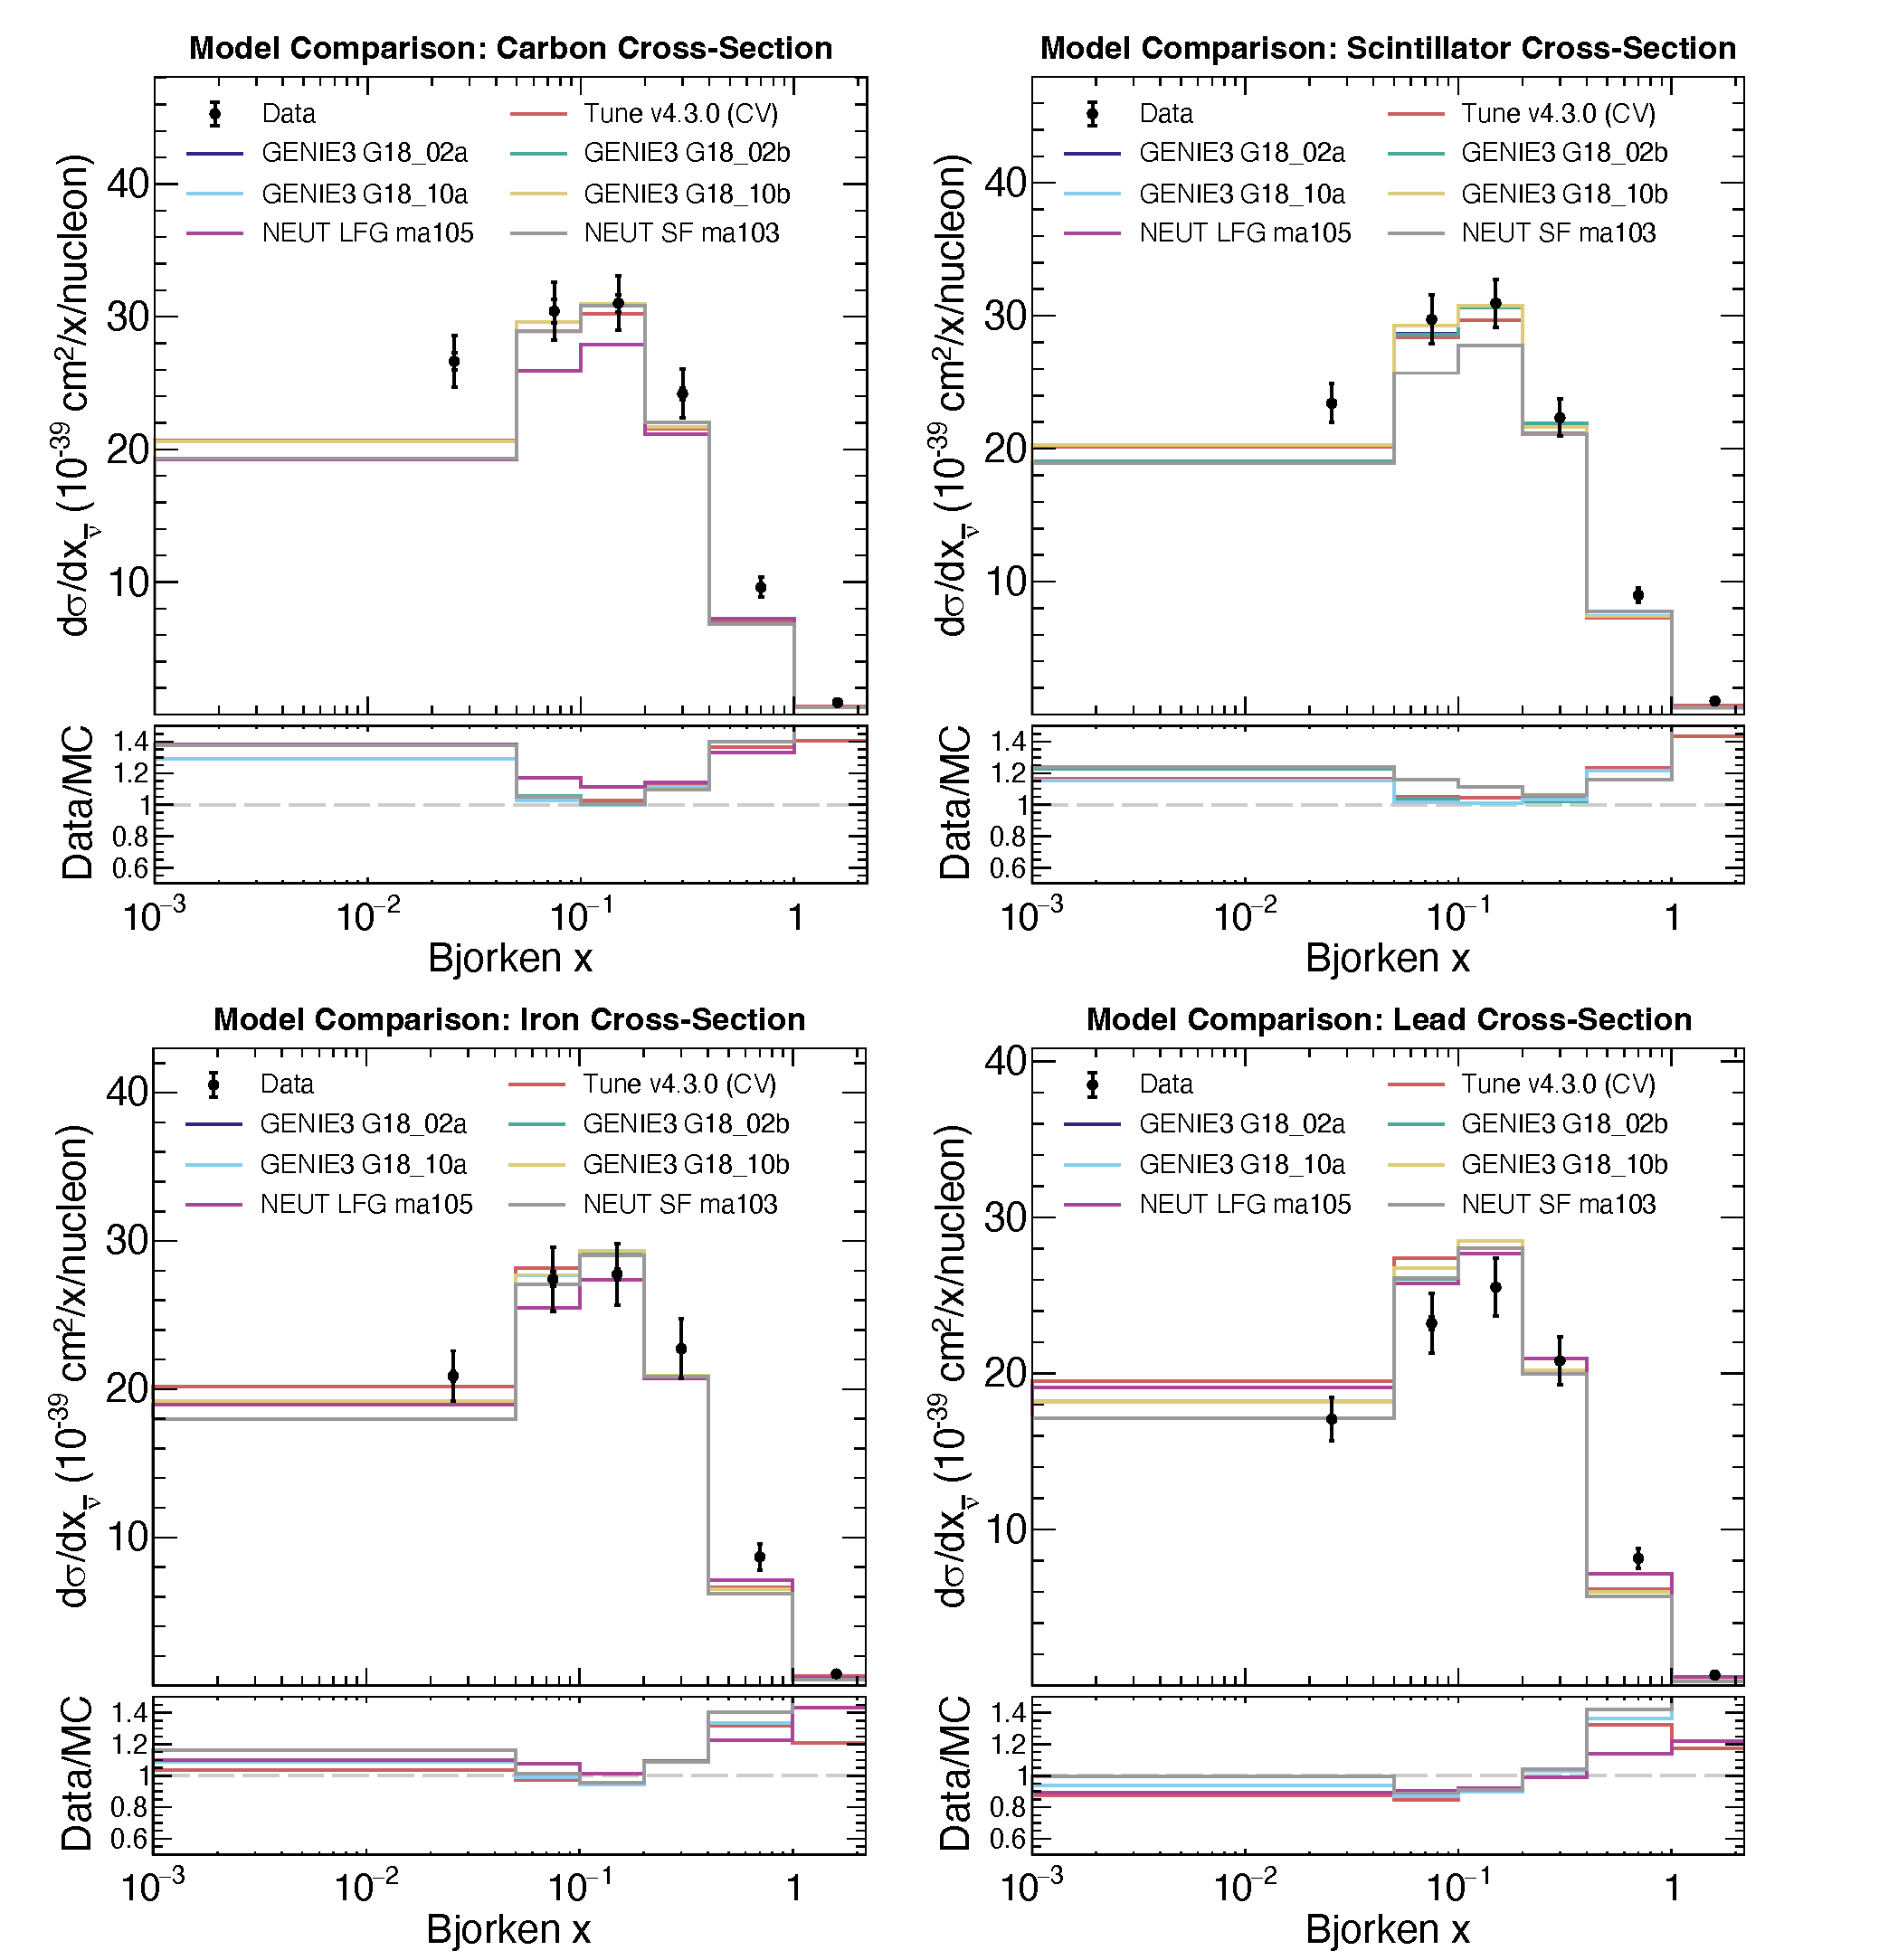
\includegraphics[width=1.\textwidth]{09results/figures/xsec_x_modelComparison.pdf}}%
    \caption{Measured carbon, scintillator, iron, and lead (from left to right, top to bottom) cross-section as a function of Bjorken $x$ compared to various antineutrino generator predictions. The inner error bar on the data indicates the statistical error while the outer error bar corresponds to the total, i.e. statistical + systematic, error. The statistical errors on the various model predictions are not shown for clarity (but they are also negligible). The bottom panel indicates the agreement between the data and various models through their respective data-to-model prediction ratios.}
    \label{fig:xsec_x_modelComparison}
\end{figure}

% bjorken x
The Bjorken $x$ cross-section results across the various nuclei prefer both NEUT implementations over GENIE 3. Specifically, the local Fermi gas model appears to perform quite well. This preference could potentially be attributed to differences in the treatment of the resonant pion production to deep inelastic scattering transition region compared to GENIE, or the distinct intranuclear cascade. However, further investigation would be required for a more detailed understanding.

% bjorken x ratio
In contrast, many of the differences between the data and the models cancel out in the Bjorken $x$ cross-section ratios to the scintillator. Consequently, GENIE 3 shows its strength in modeling the $A$-dependence of the overall cross-section again. Both G18\_02a/b and G18\_10a/b predict the suppression in the low-$x$ region relatively well, with the Pb/CH ratio requiring additional strength, similar to the $p_{\text{T}}$ ratios.

\begin{figure}[t!] 
    \centering
    {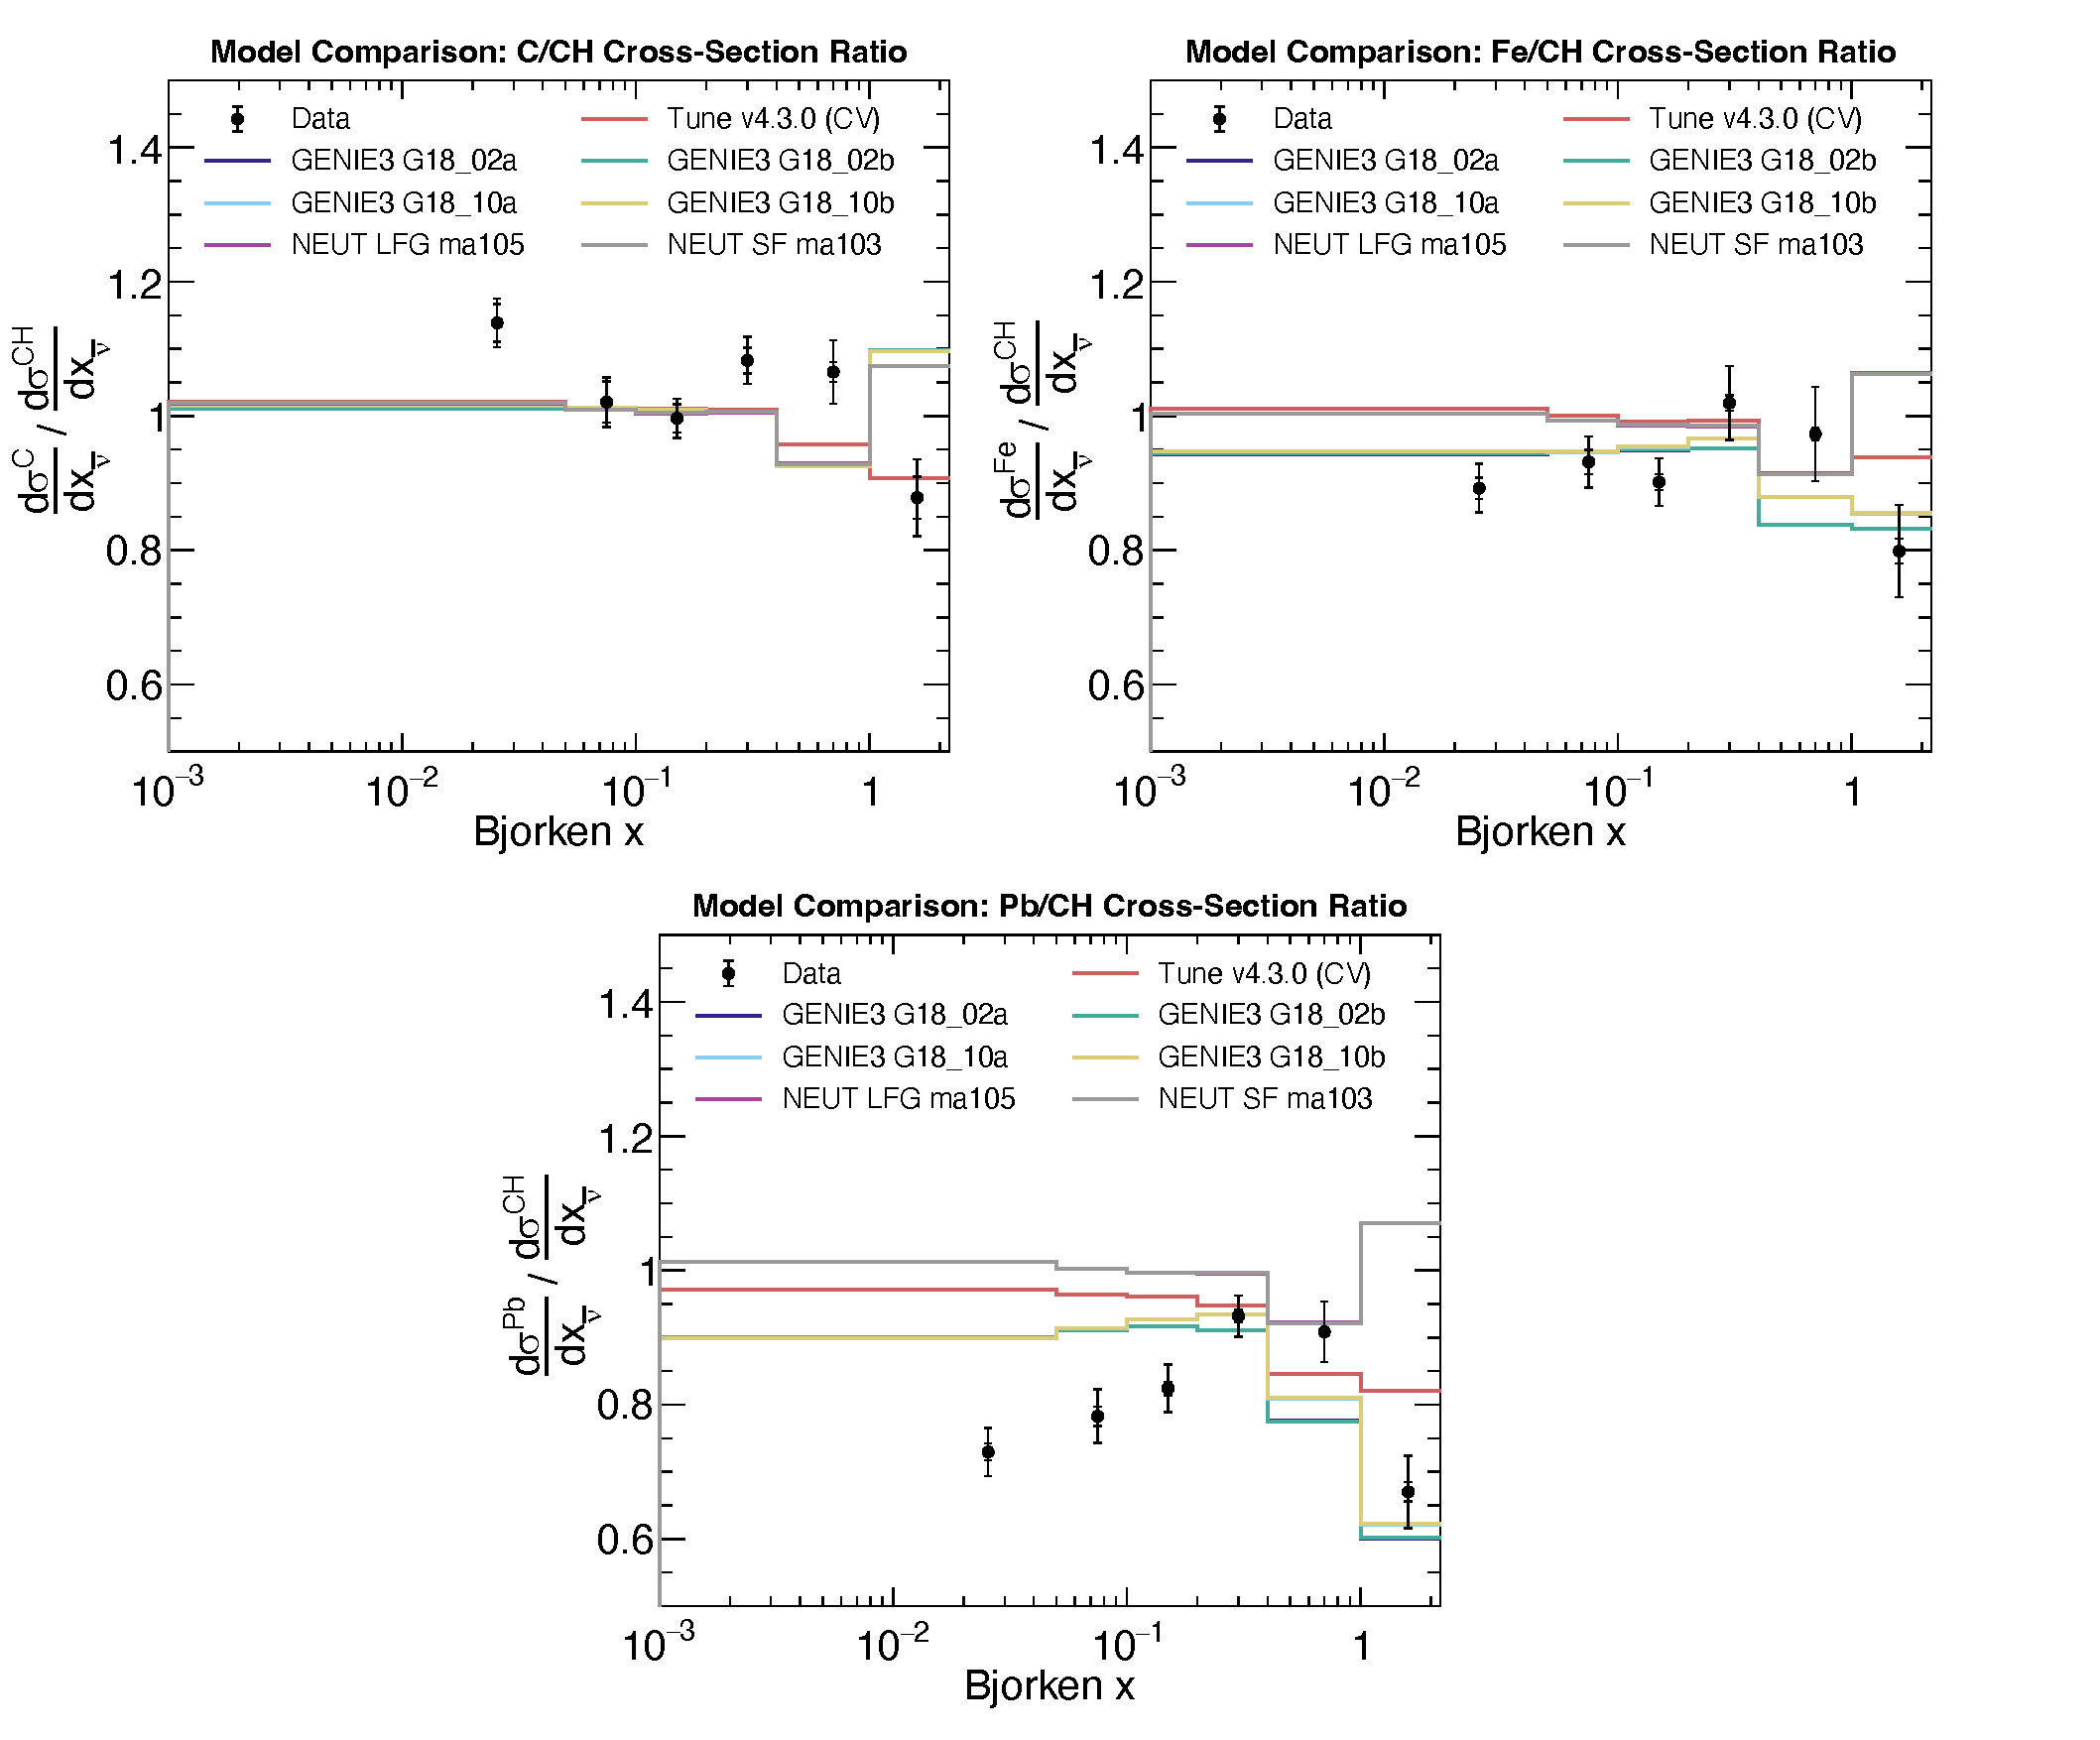
\includegraphics[width=1.\textwidth]{09results/figures/ratios_x_modelComparison.pdf}}%
    \caption{Measured carbon-to-scintillator (top left), iron-to-scintillator (top right), and lead-to-scintillator (bottom) cross-section ratios in Bjorken $x$ are compared to various antineutrino generator predictions. The data is displayed with both the statistical (inner error bars) and the total (outer error bars) uncertainty. The suppression predicted by the GENIE 3 models at low Bjorken $x$ attempts to follow the shape of the data.}
    \label{fig:ratio_x_modelComparison}
\end{figure}

\begin{table}[b!]
    \vspace{-18pt}
    \centering
    \begin{adjustbox}{width=1.01\textwidth,center=\textwidth}
    \begin{tabular}{c  c c c c c c c}
    \hline \\ [-1.5 ex]
    \multirow[c]{2}{*}{Cross-section} & \multicolumn{7}{c}{Model $\chi^2$/ndf for Bjorken $x$ cross-section (ndf = 6) } \\ [0.8ex]
    & CV & G18\_02a & G18\_02b & G18\_10a & G18\_10b & LFG\_ ma105 & SF\_ma103\\ [0.5ex] % inserts table %heading
    \hline
    \hline \\[-1.9ex]
    Carbon & 5.34 & 8.44 & 8.47 & 7.02 & 7.07 & 4.47 & 8.44\\
    %\hline
    Iron & 3.50 & 7.64 & 7.64 & 5.98 & 6.10 & 2.07 & 7.64 \\
    %\hline
    Lead & 4.46 & 5.94 & 5.92 & 5.19 & 5.23 & 1.27 & 5.94 \\
    %\hline
    Scintillator & 17.22 & 44.61 & 44.30 & 29.79 & 30.12 & 10.49 & 10.49 \\
    \hline
    \end{tabular}
    \end{adjustbox}
    \caption{Fully correlated $\chi^2$/ndf calculated according to Equation~\ref{eq:fullyCorrelatedChi2} to evaluate the agreement between the measured data and the various models for carbon, scintillator, iron, and lead cross-section in Bjorken $x$. Note that the relatively large $\chi^2$/ndf for the scintillator is attributed to the large statistics of the sample. The first numerical column indicates the agreement with the underlying simulation prediction.}
    \label{table:xsec_modelComparison_x}
\end{table}
\clearpage
\begin{table}[t!]
    \centering
    \begin{adjustbox}{width=1.01\textwidth,center=\textwidth}
    \begin{tabular}{c c c c c c c c}
    \hline \\ [-1.5 ex]
    \multirow[c]{2}{*}{Cross-section ratio} & \multicolumn{7}{c}{Model $\chi^2$/ndf for Bjorken $x$ (ndf = 6) } \\ [0.8ex]
     & CV & G18\_02a & G18\_02b & G18\_10a & G18\_10b & LFG\_ ma105 & SF\_ma103\\ [0.5ex] % inserts table %heading
    \hline
    \hline \\[-1.9ex]
    C/CH & 5.91 & 5.80 & 5.85 & 5.73 & 5.71 & 5.60 & 5.53 \\
    %\hline
    Fe/CH & 6.28 & 3.39 & 3.47 & 3.01 & 3.08 & 9.95 & 9.91 \\
    %\hline
    Pb/CH & 12.69 & 11.14 & 11.13 & 7.74 & 7.69 & 20.19 & 20.24 \\
    \hline
    \end{tabular}    
    \end{adjustbox}
    \caption{Fully correlated $\chi^2$/ndf calculated according to Equation~\ref{eq:fullyCorrelatedChi2} to assess the agreement between the measured data and the various models in the cross-section ratios to scintillator for carbon, iron, and lead in Bjorken $x$. The first numerical column indicates the agreement with the underlying simulation prediction.}
    \label{table:xsecRatio_modelComparison_x}
\end{table}

% tunes in the appendix
Finally, various MINERvA results are also reported with different MINERvA tunes applied to the base GENIE 2.12.6, i.e. tunes different from the underlying v4.3.0~used in this analysis. To enable further review of the results of this analysis in the context of other MINERvA results, the comparisons of the measured cross-sections and cross-section ratios are included in Appendix~\ref{ch:appendix_tuneComparisons}. 

\section{Extension to two dimensions}
\label{sec:analysis2D}

%\section{Differences compared to 1D}
%\section{2D Cross-section distributions}
%\section{2D Cross-section ratios}



% some other notes
%In summary, these data on single pion production on a wide variety of nuclei provide a new way to test nuclear models through their nuclear dependence. We observe a large modification to the predicted Q2 distribution of single pi+ events that it can be consistently seen in all nuclei. These results give guidance in how the wealth of data on scintillator targets can be applied to models for oxygen and argon for future neutrino experiments.
    
% Combined with other measurements from MINERvA
% These measurements combined provide key benchmarks for the field’s description of how the nucleus impacts neutrino interactions
    

%It has been experimentally demonstrated that the structure of the nucleon in the nuclear environment is indeed different than the free nucleon structure. Understanding this modified structure has played an important part in the experimental and theoretical exploration of nucleon structure by neutrinos and is one of the important goals of the on-going MINERvA experiment at Fermilab.
    
    
